\RequirePackage{fix-cm}
%
%\documentclass{svjour3}                     % onecolumn (standard format)
%\documentclass[smallcondensed]{svjour3}     % onecolumn (ditto)
\documentclass[smallextended]{svjour3}       % onecolumn (second format)
%\documentclass[twocolumn]{svjour3}          % twocolumn
%
\smartqed  % flush right qed marks, e.g. at end of proof
%
\usepackage{graphicx}
 \usepackage{booktabs}
\usepackage[caption=false]{subfig}
 \usepackage[colorinlistoftodos,backgroundcolor=yellow]{todonotes} %disable
 \usepackage{color}

\usepackage{balance}

\newcommand{\XXX}[1]{\textcolor{red}{{\it \textbf{[XXX: #1]}}}}
\hyphenation{Max-DB data-base}

\usepackage{comment}
\newtheorem{mydef}{definition}
\newcommand{\slbl}[1]{\textbf{\textsf{#1}}}
\usepackage{multirow}%,multicolumn}
\usepackage{slashbox}
\usepackage{wrapfig}
\usepackage{booktabs, colortbl}
\usepackage{amsmath}
\usepackage{url}
\usepackage[pdfstartview=FitH,bookmarksopenlevel=3,bookmarks=true]{hyperref} %pdfpagescrop={92 112 523 778},
\journalname{Empirical Software Engineering}

\begin{document}

\title{Automated Topic Naming}
%\thanks{Grants or other notes
%about the article that should go on the front page should be
%placed here. General acknowledgments should be placed at the end of the article.}

\subtitle{Supporting Cross-project Analysis of Software Maintenance Activities}
%\titlerunning{Short form of title}        % if too long for running head

%\numberofauthors{4}

\author{
Abram Hindle \and
Neil A. Ernst \and
Michael W. Godfrey \and
John Mylopoulos
}
%\authorrunning{Short form of author list} % if too long for running head

\institute{
  Abram Hindle \at 
  Dept. of Computing Science\\
  University of Alberta\\
  Edmonton, AB, CANADA\\
  \email{abram@softwareprocess.es}
\and
  Neil A. Ernst \at
  Dept. of Computer Science\\
  University of British Columbia\\
  Vancouver, BC, CANADA\\
  \email{nernst@cs.ubc.ca}
\and
  Michael W. Godfrey \at
  David Cheriton School of Computer Science\\
  University of Waterloo\\
  Waterloo, Ontario, CANADA\\
  \email{migod@uwaterloo.ca}
\and 
  John Mylopoulos \at
  Dept. Information Eng. and Computer Science\\
  University of Trento\\
  Trento, ITALY\\
  \email{jm@disi.unitn.it}
}

\date{Received: date / Accepted: date}
% The correct dates will be entered by the editor


\maketitle

\begin{abstract}

%Researchers have employed a variety of techniques to extract underlying
%topics that relate to software development artifacts.  Typically, these
%techniques use semi-unsupervised machine-learning algorithms to suggest
%candidate word-lists, topics.  
Software repositories provide a deluge of software artifacts to
analyze. Researchers have attempted to summarize, categorize, and relate these
artifacts by using semi-unsupervised machine-learning
algorithms, such as Latent Dirichlet Allocation (LDA), used for concept and topic analysis to suggest candidate
word-lists or topics that describe and relate software artifacts.
However, these word-lists and topics are
difficult to 
interpret in the absence of meaningful summary labels.  Current topic modeling 
techniques assume manual labelling and do not use domain-specific knowledge
to improve, contextualize, or describe results for the developers.  
We propose a solution: \emph{automated labelled topic extraction}.
  Topics are extracted 
using  LDA from commit-log comments recovered
from source control systems. % such as CVS and BitKeeper.  
These topics are given labels from a generalizable
cross-project taxonomy, consisting of non-functional
requirements. Our approach was evaluated with experiments and case studies
on three large-scale Relational Database Management System (RDBMS) projects: MySQL, PostgreSQL and MaxDB.  
The case studies
show that labelled topic extraction can produce appropriate,
context-sensitive labels that are relevant to these projects, and provide fresh
insight into their evolving software development activities.
%160 words
\keywords{ Software maintenance \and Repository mining \and Latent Dirichlet allocation \and Topic models}

\end{abstract}

\section{Introduction}
A key problem for practicing software maintainers is gaining an
understanding of \emph{why} a system has evolved the way it has \cite{Mockus00}. 
This is different from \emph{how} a system has evolved. 
% NE this phrase confuses me: "because the change of behaviour itself is the \emph{how}.
Looking back on streams of artifacts scattered across different
repositories, inferring what activities were performed, when, and for
what reasons, is hard without expert advice from the developers
involved. 
%new stuff
% edit this. awkward
In this work we provide a method of automatically labelling  development topics extracted from commit logs called \emph{labelled topic extraction}.


Concrete applications of \emph{labelled topic extraction} include the annotation of development artifacts with NFR-related tags and the creation of project dashboards.  Annotating software development artifacts with NFR-related tags would allow developers to create detailed directed queries of different artifact kinds that concern the same NFR; for example, a developer could browse the recent history of performance-related bug reports and code check-ins. Project dashboards distill detailed information about a software system into a simpler and more abstract view that summarizes key aspects of the development effort \cite{dashboard}; labelled topic extraction would allow managers to track effort related to specific NFR topics, such as \emph{usability} or \emph{portability}.


Topic modeling (such as Latent Dirichlet Allocation ~\cite{Blei2003}) is a machine learning technique that creates
multinomial distributions of words extracted from a text corpus. 
This technique infers the hidden structure of a corpus using posterior
inference: the probability of the hidden structure given the data. 
Topic models are useful in software maintenance because they summarize
the key concepts in a corpus -- such as source code, commit comments, or
mailing-list messages -- by identifying words that commonly occur together. 
Among other uses, topic modelling can quickly give developers an overview of where significant
activity has occurred, and provide managers or maintainers an enhanced understanding of the project's 
history.

%migod
While machine learning techniques can automatically identify clumps of
commonly recurring terms, devising an appropriate summary label for
each clump/topic is harder.  
A given topic extracted from a set of commit logs might consist of the following terms: \emph{ ``listener change remove add fire''}. 
This topic might reasonably be labelled as
\emph{``event handling''} by a developer who understands the domain well,
despite the fact that this label does not appear in the word list itself.  
Current approaches to topic labelling rely on manual intervention by
human experts, and also are limited to project-specific topic labels.  
In this paper, we introduce \emph{labelled topic extraction}, an
approach that automatically suggests project-independent labels for topics.

%migod
In general, the fruits of mining software artifacts are often project
specific and hard to generalize.  
However, in our previous work we
investigated \emph{topic trends} --- that is, topics that recur over
time --- we observed that topic trends often corresponded to
non-functional requirements (NFRs)~\cite{Hindle09ICSM}, which is
further emphasized in this paper due to the large numbers of NFR
labelled topics.  
This is encouraging, as NFRs have the property of being cross-domain
and widely applicable. 
In this sense, they are useful abstractions for developer
conversations about different software projects.  
Furthermore, there is a series of standards on NFRs, such as ISO9126 \cite{iso9126}, that are specifically intended to apply to projects of varying
types; this suggests that our goal of trying to extract NFR-related development topics, such as those related to software quality models, holds promise.

In this paper, we describe \emph{automated labelled topic extraction}. It addresses two gaps in the topic mining literature:
\begin{enumerate}
  \item Topic mining of software has been limited to one project at a time. 
This is because traditional topic mining techniques are specific to a particular data-set. 
\textit{Automated labelled topic extraction} allows for comparisons \textit{between} projects. 
  \item Topic modeling creates word lists that require interpretation by the user to assign meaning. 
Like (1), this means
that it is difficult to discuss results independent of the project context. 
Our technique automatically, or with some initial training, assigns labels across projects.
\end{enumerate}

This paper makes the following contributions: 
\begin{itemize}
\item We introduce the concept of labelled topic extraction, using a taxonomy of non-functional requirements (NFR) for our labels; 
\item We evaluate three kinds of automatic topic labelling methods:
  semi-unsupervised labelling  of topics (word-lists), supervised labelling of
  topics with a single NFR (machine learning), 
  and supervised labelling of topics with multiple NFRs (multi-label
  machine learning);
\item We examine how NFRs correlate with the work of individual developers;
\item We provide a method of cross-project analysis via topic labelling, and
we apply these techniques to visualize NFRs over time, and to analyze maintenance activities.

\end{itemize}

%We first introduces labelled topic extraction, and then uses that technique to analyze development activity in two large-scale examples.
We begin by discussing related work in Section \ref{sec:related}.
Next, we describe how we generated our data (Section \ref{sec:wordlist}). For semi-unsupervised classification (Section \ref{sec:unsuplabelling}), we
begin by creating word-lists to signify when a topic matches an NFR label. We then apply our classifier and analyze the results. 
%and how we created the word-lists used in unsupervised classification. 
%We show that labels with their topics can be learned and used to classify other data-sets, either without training 
%Our goal is to label a given topic with either an NFR from our taxonomy,
 %Section \ref{sec:unsuplabelling} presents our technique for using word-lists to do unsupervised classification, and describes the results.

This work extends our previous work~\cite{msr2011}. The major extensions in this paper are as follows:
\begin{itemize}
	%\item We added new results on developer activities.
	\item We conducted another case-study on PostgreSQL. 
	\item We used two authors to each annotate the same PostgreSQL topics in order to compare
these annotations. 
	\item We used this new case-study to test inter-rater reliability, described in Section \ref{sec:inter-rater}. 
	\item We conducted an analysis of PostgreSQL authors and their association with NFRs and
topics (Section \ref{sec:developers}).
\end{itemize}


In Section \ref{sec:suplabelling}, we manually annotate the topics, and use those annotations as training data for supervised classification.  
%We then present visualizations of named topics and their trends over time to aid communication and analysis. 
To demonstrate an application of labelled topic extraction, we use an exploratory case study of three open source database systems to show how named
topics can be compared between projects  (Section \ref{sec:analysis}). 
The paper concludes with a discussion of limitations (Section \ref{sec:limit}), and future work.


\section{Previous Work}
\label{sec:related}

The idea of extracting higher-level \emph{concerns} and \emph{topics}, also known as
 \emph{concepts}, \emph{aspects} or \emph{requirements},
has been approached from documentation-based and repository-based
perspectives.

Cleland-Huang and her colleagues have investigated mining requirements
documents for non-functional requirements (NFR) (software
qualities)~\cite{Cleland-Huang2006}.  
%Their approach is similar to
%ours, as they mine keywords from NFR catalogues.  They differ from our approach because
%they mine requirements documents whereas we mine revisions.
One approach they tried was similar to this one, with keywords mined from NFR catalogues found in Chung et al.~\cite{corollary99}. 
Their approach resulted in a recall of $80\%$ with precision of $57\%$ for the \emph{security} NFR, but could not find a reliable source of keywords for other NFRs. 
Instead, they developed a supervised classifier by using human experts to identify an NFR training set. 
Our research is different because we use a more comprehensive set of terms based on a taxonomy that is an integral part of our framework.
Another difference is that we make cross-project comparisons instead of focusing
on a single project.
They relied on relatively well-structured requirements documents instead of version control histories that we use.
The objective of Cleland-Huang's study was to identify new NFRs for system development, 
while our objective was to recover those latent NFRs from commit-log messages of the project. 

%There are several reasons we did not follow this route. 
%One, we believe we have a more comprehensive set of terms due to the taxonomy we chose. 
%Secondly, we wanted to compare across projects. 
%Their technique was not compared across different projects and the applicability of the training set to different corpora is unclear. 
%A common taxonomy allows us to make cross-project comparison. 
%Although subject to the assumption that all projects conceive of these terms in the same way.
%Thirdly, while the objective of Cleland-Huang's study was to identify new NFRs (for system development) 
%our study assumes these NFRs are latent in the commit-log messages of the project. 

Similarly, Mockus and Votta~\cite{Mockus00} studied a large-scale industrial change-tracking system. 
Mockus and Votta leveraged WordNet~\cite{Fellbaum1998}, an English-language ``lexical database'' that contains semantic relations between words,
including common related forms (similar to word stemming), meronymy and synonymy.
They used WordNet for word roots as they felt the synonyms would be
non-specific and cause errors.
%, problems we also encountered. 
Mockus et al. validated their labels with system developers.
Since we study multiple projects, instead of a single project, these
kind of interviews were not feasible (particularly in the distributed world of open-source software).

Another approach is to extract concerns from software repositories.
Marcus et al.~\cite{marcus04wcre} used Latent Semantic Indexing (LSI)
to identify commonly occurring concerns for software maintenance. 
The
concerns are given by the user, and LSI is used to retrieve them from
a corpus. 
Topic modelling generates topics that are independent of a user query, and relate only to word frequencies in the corpus.
%Some results were interesting, but their precision was quite low. 

With ConcernLines, Treude et al.~\cite{treude09cl} showed tag occurrence
using colour and intensity, and our plots that rely on color and intensity
have a similar look and feel to Treude et al.'s plots.
They mined
developer created 
change request tags from IBM Jazz
repositories and used these 
in order to analyze the evolution of a single product.
Change requests in Jazz allow for users to annotate each change
request and check-in with tags such as ``ui'', ``usability'' or
``milestone 3''. 
% make evolutionary analyses of a single product. 
The presence of a well-maintained set of tags is obviously essential to the success of this technique.

%XXXXXXXXXXXX OPTIONAL
% Not sure we need this
%Mens et al.~\cite{mens08icsm} conducted an empirical study of Eclipse, a popular Java IDE, to verify the claims of Lehman~\cite{lehman97sms}.
% They concerned themselves with source code only, and found Law Seven, ``Declining Quality'', to be too difficult to assess:
% ``[we lacked an] appropriate measurement of the evolving quality of the system as perceived by the users \cite[p. 388]{mens08icsm}''. 
%This paper examines the notions of quality in terms of a consistent ontology, as Menset al. call for in their conclusions.

% in our previous work~\cite{Hindle09ICSM}, as well as -- CITED a little too often (vanity cites!)
In Baldi et al.~\cite{Baldi2008}, topics are named manually: human
experts read the highest-frequency members of a topic and assign a
label accordingly. 
%XXX Possible to cut this
As discussed earlier, given the topic \emph{``listener change remove add fire''}, Baldi et al. would assign the label \emph{event-handling}. 
The labels are reasonable enough, but still require an expert in the field to determine them. 
Furthermore, these labels are project-specific, because they are
generated from the data of that project. For example we might have a label called \emph{`Oracle'}
in the MySQL case, since Oracle owns MySQL. 
%We do this differently.
%This paper does this differently. 
Our approach differs: first of all, we automate the process of naming the topics; secondly, we label topics with project-independent terms, in order
to permit cross-project comparison.

Mei et al.~\cite{Mei2007} use context information to automatically name topics. 
They describe probabilistic labelling, using the frequency distribution of words in a topic to create a meaningful phrase. 
They do not use external domain-specific information as we do, but we
do not generate phrases from the topics.


%Massey~\cite{massey02icse} and Scacchi~\cite{scacchi02,scacchi05b} looked at the topic of requirements in open-source software. 
% this reduces the line length and drops a ref even though we still have a scacchi kickin around
Massey~\cite{massey02icse} and Scacchi~\cite{scacchi05b} looked at the topic of requirements in open-source software. 
Their work discusses the source of the requirements and how they are used in the development process. 
 German~\cite{german03gnome} looked at GNOME specifically, and listed several sources for requirements: leader interest, mimicry, brainstorming, and prototypes. 
None of this work  addressed quality requirements in OSS, nor did it examine requirements trends.
% NE 0113 this seems too early to mention 'result'.
In Hindle et al. \cite{Hindle2007} we examined release patterns in OSS. That work showed that there is a difference between projects regarding maintenance
techniques. This supports the result described in this paper, that software qualities are not discussed with the same frequency across projects.



This paper and our MSR 2011 paper~\cite{msr2011} are based off of the
work of Ernst and Mylopoulos~\cite{ernst10refsq} and the work of Hindle et
al.~\cite{Hindle09ICSM}.
In Ernst and Mylopoulos~\cite{ernst10refsq}, we describe an earlier
project that identifies changes in quality requirements
in GNOME software projects (GNOME is a Linux desktop environment). Unlike this paper, this earlier approach was more exploratory and had
less validation. In particular, it  uses different word-lists, solely uses text-matching,
and does not leverage machine learning strategies.  
Our approach in this paper, and our
MSR 2011 paper~\cite{msr2011}, extends Ernst and Mylopoulos~\cite{ernst10refsq} by using 
word-lists to label topics, which are completely absent in the earlier work.
 Hindle et
al.~\cite{Hindle09ICSM}
 propose a windowed method of topic
analysis that we extend with labelled
topics, NFRs and new visualizations. This windowed method was
to bucket documents  by time windows (such as months), that could overlap if
necessary, and then use LDA to extract documents from these
bucket. These topics were then related to topics in other adjacent
buckets, and joined if deemed sufficiently similar. This paper, and our
MSR'2011 paper~\cite{msr2011}, extend the method of Hindle et
al.~\cite{Hindle09ICSM} by labelling topics
and providing an alternative visualization, the topic time-line
described in Section \ref{sec:analysis}.




\section{Study Design and Execution}
Figure \ref{fig:process} gives an outline of our methodology.
We begin by gathering source data and creating topic models. For semi-unsupervised labelling, we generate three sets of word-lists as signifiers for NFRs.
%e created labels using a well-known NFR taxonomy. 
With supervised learning, we train our data with manual annotations in order to match topics with NFRs. Finally, these topics are used to analyze the
role of NFRs in software maintenance.

\begin{figure}
  \centering
 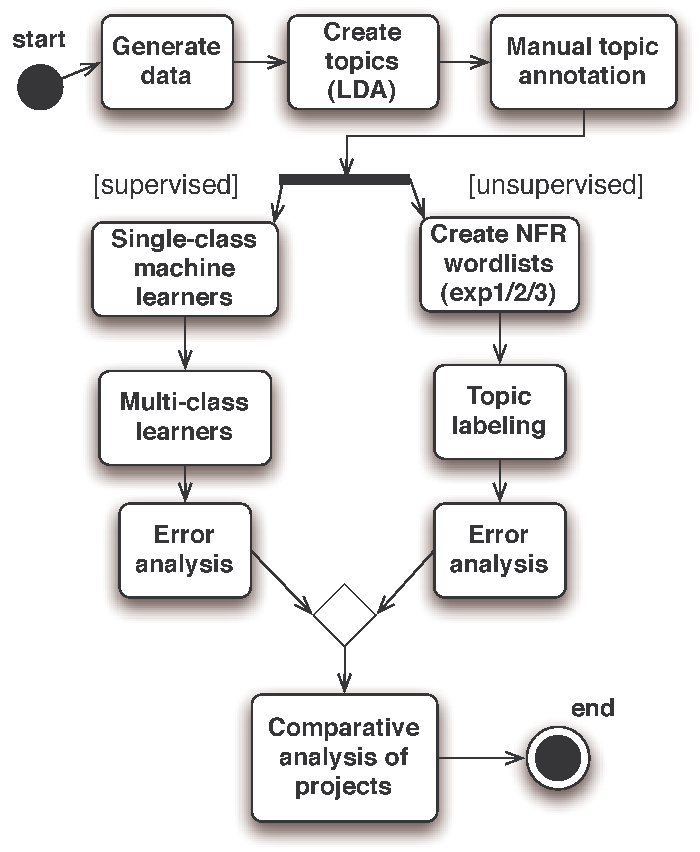
\includegraphics[height=.6\textheight]{figures/process-model}
 \caption{Research methodology process view.}
  \label{fig:process}
\end{figure}

\subsection{Generating the Data}
\label{sec:wordlist}

To evaluate our approach, we sought candidate systems that were mature projects and had openly accessible source control repositories. 
We selected systems from the same application domain, to control for differences in functional, rather than non-functional, requirements. 
We used three different open-source, partially-commercial database systems:
\begin{itemize}
\item  MySQL 3.23. Started in 1994 and MySQL 3.23 was released in early 2001. MySQL contains $320,000$ lines of C and C++ source code~\footnote{generated
using David A. Wheeler's \emph{SLOCCount},
{http://dwheeler.com/sloccount}.}. We used the MySQL 3.23 source control  history from July
31st, 2000 to August 9th, 2004.
\item MaxDB 7.500. Started in the late 1970s as a research project, and was later acquired by SAP. As of version 7.500, released April 2007, the project
has over $940,000$ lines of C source
code~\footnote{{http://www.sdn.sap.com/irj/sdn/maxdb}}. 
 We used the MaxDB 7.500 source control history from June
29th, 2004 to June 19th, 2006.
\item PostgreSQL 7.3. Started in the 1980s as a Berkeley research
  project~\footnote{{http://www.postgresql.org/docs/7.3/static/}}. PostgreSQL
  7.3 contains $306,000$ lines of C code.
 We used the PostgreSQL 7.3 source control  history from May 9th, 2002 to 
 August 26th, 2004.

\end{itemize}
  
%Choosing an older version of these projects allowed us to focus on projects which have moved further into the maintenance phase of the software life-cycle.
We explicitly chose older versions of mature projects from a stable problem domain to increase the likelihood that we would encounter primarily
maintenance activities in our studies. We felt that a single domain
would allow for cross-project comparison. At the same time we
recognize that a problem-domain alone does guarantee functional and
non-functional similarity.
For instance each database system has a different focus, PostgreSQL
tends to focus on fulfilling much of the SQL92 specification and adding
more features while MySQL has been slow to adopt much of the spec.
 As a consequence our choice of looking at a
single domain limits our generalizability. What we show in this paper
will be somewhat biased towards database software.

For each project, we used source control commit comments, the messages
that programmers write when they commit revisions to a source control
repository. 
Most commits we observed had commit comments (90\% in MySQL 3.23,
98.5\% in PostgreSQL and 99.99\% in MaxDB 7.500).
Commit comments are often studied by researchers, as they are the most readily accessible source of project interactions, and developers are often
required to create them by the repository mechanism (e.g., Git).  Additionally, relying only on commit comments makes our approach more generalizable,
as we do not assume the presence of other artifact corpora.
%This is the most readily accessible source of project interactions for outside researchers, since developers often or always (e.g., Git) write such
%message. Our approach is more generalizable if it does not assume the presence of other corpora. 
%bug trackers and email-list archives were not available for both projects. 
An example of a typical commit message, from MySQL, is: \textit{``history annotate diffs bug fixed (if mysql\-\_real\-\_connect() failed there were
two pointers to malloc'ed strings, with memory corruption on free(), of course)''}. 
We extracted these messages and indexed them by creation time. 
Each word in the message was
stripped of punctuation and converted to lowercase.
We summarized each message as a word distribution minus stop-words
such as ``\emph{the}'' and ``\emph{at}''. We did not stem or apply any
other transforms to the messages.
Our stop words are derived from the Natural Language Toolkit (NLTK) stop-word English stop-word
list~\footnote{NLTK: \url{http://www.nltk.org/}.

%Stemming was performed in the later stages of our analysis. % WAS IT?

For the commit message data-sets of each project, we created an XML file that separated commits into 30 day periods. 
%This size of period, 30 days, is smaller than the time between minor
%releases but large enough for there to be sufficient commits to
%analyze
We chose a period size of 30 days as it is smaller than the time between minor releases but large enough for there to be sufficient commits to
analyze~\cite{Hindle09ICSM}. 
For each 30 day period of each project, we input the messages of that period into Latent Dirichlet Allocation (LDA), a topic analysis
algorithm~\cite{Blei2003}, and recorded the topics the algorithm extracted.
%For each project and for each period of messages a project, we input these messages 
%we created `topics' using Latent Dirichlet Allocation, a topic identification algorithm. 

A topic analysis tool such as LDA will try to find $N$ independent
word distributions within the word distributions of all input
messages. 
If there are not $N$ independent word distributions, the topics
produce tend to be duplicates of each other, that is they share the
top terms. During this study we found that when $N$ was 20 we did not
witness duplicate topics very often.
Linear combinations of these $N$ word distributions are meant to represent and recreate the word distributions of any of the original messages. 
These $N$ word distributions effectively form \emph{topics}: cross-cutting collections of words relevant to one or more of our commit messages. 
LDA extracts topics in an unsupervised manner; the algorithm relies
solely on the source data and word distributions of messages, with no human intervention.

In topic analysis a single document, such as a commit message, can be related to multiple topics. 
Representing documents as a mixture of topics maps well to source code repository commits, which often have more than one purpose~\cite{Hindle09ICSM}.  
For this paper, a topic represents a word distribution generated from a group of commit log comments which are related by their content.  
%In this paper a topic is a set of tokens extracted from commit messages found within a project's source control system (SCS).

We applied Blei's LDA implementation~\cite{Blei2003} against the word distributions of these commits, and generated lists of topics per period. 
We set the number of topics to generate to $20$, because past experimentation showed that fewer topics might aggregate multiple unique topics while
any more topics dilutes the results and creates indistinct topics~\cite{Hindle09ICSM}. 
% Furthermore, more than $20$ topics quickly became infeasible for inspection.

\subsubsection{The High-level Labels}

%\noindent \textbf{The high-level labels} --- 

To facilitate cross-project comparison, we used a taxonomy of NFRs. This taxonomy is based on the ISO quality model, ISO9126~\cite{iso9126}. 
ISO9126 describes six high-level NFRs: \emph{maintainability, functionality,
portability, efficiency, usability,} and \emph{reliability}
%\footnote{While there may be lingering debate in some circles about these terms, an ISO standard
%seems like a reasonable starting point for our work.}.
There is some debate about the terms in this model, and whether they are a) the correct terms and b) correctly organized. 
However, ISO9126 is ``an international standard and thus provides an 
internationally accepted terminology for software quality
\cite[p. 58]{Boegh2008},'' that is sufficient for the purposes of this
research.  
\emph{Performance} is an example of RDBMS word related to the \emph{efficiency} NFR.
We claim that these NFRs are maintenance concerns (to varying degrees) in all software projects, and are therefore well-suited for comparisons between
projects.

%\noindent \textbf{Creating a validation corpus} --- 

\subsubsection{Creating a Validation Corpus}
To evaluate both semi-unsupervised and supervised classification, we
created a validation set of manually labelled topics. For each project,
 the annotators (the first two authors) annotated each extracted topic in each period with
the six NFR labels listed above.
Annotators did not annotate each other's annotations, but some brief
inspection of annotations was used to confirm that the annotators were
acting similarly. PostgreSQL (PgSQL) was annotated by both annotators in order
to evaluate inter-rater reliability.
We looked at each period's topics, and assessed what the data ---
consisting of the frequency-weighted word lists and messages ---
suggested was the label for that topic. 
We were able to pinpoint the appropriate label using auxiliary information as well, such as the actual revisions and files that were related to the
topic being annotated.
For example, for the MaxDB topic consisting of a message ``exit() only
used in non NPTL LINUX Versions'', we tagged that topic
\emph{portability}. 
Given the top-level annotations of \emph{none}, \emph{portability},
\emph{efficiency}, \emph{reliability}, \emph{functionality},
\emph{usability}, and \emph{maintainability}, the annotators annotated each topic
with the relevant label. Sometimes they used finer-grained
annotations that would be aggregated up to one of these higher-level labels.
%We compared against this data-set, but we also used the data-set for our supervised machine learning based topic classification. 
% A topic may have more than one matching keyword. % ok what?

We validate classification performance using the area under the curve
of Receiver Operating
Characteristic~\cite{Fawcett2006861},
abbreviated \emph{ROC}, sometimes called \emph{AUC}, and the
F-measure, which is the harmonic mean of precision and recall, i.e.,
$2 * (P * R) / (P + R)$. 
Throughout the paper we will provide F-measure scores so that readers
who are more familiar with F-measure than ROC can intuitively
interpret the results.

ROC values provide a score %, similar to school letter-grades (A is 0.9, C is 0.6),
 reflecting how well a particular learner performed for the given data. 
ROC maps to the more familiar concepts of precision/sensitivity and recall/specificity: it plots the true positive rate (sensitivity) versus the false
positive rate (1 - specificity). 
A perfect learner has a ROC value of $1.0$, reflecting perfect recall and precision. 
A ROC result of $0.5$ would be equivalent to a random learner (that
is, issuing as many false positives as true positives). While we
recognize that using $0.5$ as the base-line means our ROC scores will
look much larger than our F-Measure scores, we feel that the knowledge
that the random selection is $0.5$ or worse is helpful for interpreting our results.
The %area under the -- NE confusing to have area again ... and not importantana
ROC of a classifier is equivalent to the probability that the classifier will rank a randomly chosen positive instance higher than a randomly chosen
negative instance.

We argue for using ROC over F-Measure because ROC suffers less from
bias than F-Measure and F-Measure often skews towards the positive
class~\cite{flach-icml03,Forman:2010:ACS:1882471.1882479}, especially
in the case of class imbalance. Forman et
al.~\cite{Forman:2010:ACS:1882471.1882479} demonstrate that cross-fold
validation will often produce low F-measures given high class
imbalance and the presence of false negatives.
Although
recent work~\cite{Forman:2010:ACS:1882471.1882479} has suggested that while ROC suffers less bias than
the average F-measure ($F_{avg}$) for cross-folds, F-measures ($F_{tp,fp}$) that are calculated from
the sums of true-positives,
false-positive, and false-negatives across folds tend to exhibit no
bias. Unfortunately our experimental framework lacks a robust way to
calculate $F_{tp,fp}$, thus we still provide ROC and $F_{avg}$.
We consider our labelling classifiers acceptable if they outperform a random classifier (0.5). 


\subsection{Semi-unsupervised Labelling}
\label{sec:unsuplabelling}

In this section we describe how to label topics based on dictionaries
mined from sources external to the projects. We call this `semi-unsupervised' because while there is no ``training set'', we do seed the wordlists manually.


\subsubsection{Generating Word Lists}

%\noindent\textbf{Generating word lists} --- 

In order to automatically label each topic with 
one of the six high-level NFRs,
%an NFR from ISO9126, 
we associate each NFR with a list
of keywords (\emph{word-lists}, in our parlance). These word-lists were determined a priori and were not extracted from the projects themselves, using the methodology explained below. In general, these lists are project and domain independent.
We intersected the words of the topics and the words of our word-lists.
We ``labelled'' a topic if any of its words matched any of the word-list's words.
A topic could match more than one NFR.
We used several different sets of word-lists for comparison, which we
refer to as \textsf{exp1}, \textsf{exp2}, and \textsf{exp3} in the text which follows. 

Our first word-list set, \textsf{exp1}, was generated using the ontology described in Kayed et al.~\cite{5072519}
That paper constructs an ontology for software quality measurement using eighty source documents, including research papers and international standards. 
The labels we used are:

\begin{quotation}
\small \noindent \textsf{
integrity, security,
interoperability, testability, maintainability, traceability,
accuracy, modifiability, understandability, availability, modularity,
usability, correctness, performance, verifiability, efficiency,
portability, flexibility, reliability.
}
\end{quotation}

Our second word-list, \textsf{exp2}, uses the ISO9126 taxonomy described above (Section \ref{sec:wordlist}) to seed the word-lists.
%We use these qualities later on as classes in supervised labelling. NE confusing the issue here, I think.
The terms from ISO9126 may not capture all words occurring in the topics that are nonetheless associated with one of the NFRs. 
For example, the term ``redundancy'' is one 
we considered to be
relevant to discussion of \emph{reliability}, but is not in the
standard. We recognize though that terms like this might be used in a
different context with a different meaning, like code-cloning.
We therefore took the NFRs from the ISO9126 and added terms to them.

To construct these expanded word-lists, we used
WordNet~\cite{Fellbaum1998}.
We then added Boehm's software quality model~\cite{Boehm+:1976:ICSE}, and classified his eleven `\emph{ilities}' into their respective ISO9126 NFRs. 
We did the same for the quality model produced by McCall et al.~\cite{mccall1977}. 
We then did a simple random analysis of mailing list messages from an open source ecosystem, KDE. Like the GNOME study we conducted in Ernst and Mylopoulos \cite{ernst10refsq}, KDE contains a suite of different products covering a variety of software categories. If we judged a given message to contain terms that were
related to one of the NFRs in ISO9126, we added it to our word-list. This allowed us to expand our word-lists with more software-specific terms.
%Finally, we randomly analyzed two mailing lists from another software project to expand our set with domain-specific terms. 
% Less info is probably better here...
%For example, we add the term ``performance'' to the synonyms for \emph{efficiency}, since this term occurs in most mail messages that discuss efficiency.
Table \ref{tbl:wnsig} shows the labels (NFRs) and word-lists we used for matching.

For the third set of word-lists, \textsf{exp3}, we extended the word-lists from \textsf{exp2} using WordNet similarity matches. 
Similarity in WordNet means siblings in a hypernym tree. 
We do not include these words here for space
considerations~\footnote{For our data repository visit \url{http://softwareprocess.es/nomen/}}. 
Wordnet similarity is a very broad match. For example, the label \emph{maintainability} is associated with
words \emph{ease} and \emph{ownership}, and the word \emph{performance} has a `sense' which refers to musical performances -- which is not related to software development. In general, as we proceed from word-lists in \textsf{exp1} to that in \textsf{exp3}, our lists become more generic.

\begin{table*}
	\centering
\begin{tabular}{c|p{9cm}}
\toprule
\textbf{Label} & \textbf{Related terms} \\
\midrule
\emph{Maintainability} &
testability changeability analyzability stability maintain maintainable modularity modifiability understandability interdependent dependency encapsulation
decentralized modular\\ \hline
\emph{Functionality} &
security compliance accuracy interoperability suitability functional practicality functionality compliant exploit certificate secured ``buffer overflow''
policy malicious trustworthy vulnerable vulnerability accurate secure vulnerability correctness accuracy\\ \hline
\emph{Portability} &
conformance adaptability replaceability installability portable movableness movability portability specification migration standardized l10n localization
i18n internationalization documentation interoperability transferability\\ \hline
\emph{Efficiency} &
``resource behaviour'' ``time behaviour'' efficient efficiency performance profiled optimize sluggish factor penalty slower faster slow fast optimization\\
\hline
\emph{Usability} &
operability understandability learnability useable usable serviceable usefulness utility useableness usableness serviceableness serviceability usability
gui accessibility menu configure convention standard feature focus ui mouse icons ugly dialog guidelines click default human convention friendly user
screen interface flexibility\\ \hline
\emph{Reliability} &
``fault tolerance'' recoverability maturity reliable dependable responsibleness responsibility reliableness reliability dependableness dependability
resilience integrity stability stable crash bug fails redundancy error failure\\ 
\bottomrule
\end{tabular}
	\caption{NFRs and associated word-lists -- \textsf{exp2}}
	\label{tbl:wnsig}

\end{table*}

\subsubsection{Automatic Labelled Topic Extraction}

%\noindent \textbf{Generating labels automatically} --- 

Using our three word-lists (\textsf{exp1}, \textsf{exp2}, \textsf{exp3}), we labelled our topics with an NFR where there was a match between a word in
the list and the same word somewhere in the frequency distribution of words that constitute the topic.
A \emph{named topic} is a topic with a match. 
\emph{Unnamed topics} occur where there is no such match. 
This may indicate either a lack of precision in the word-lists, or simply that this topic is not associated with non-functional
requirements.
All experiments were run on the data-sets for each project (e.g., PostgreSQL, MySQL, MaxDB). LDA
extracted $20$ topics per period for each project.
% Is this good enough
Each change-log message was lightly processed before applying LDA:
words were converted to lowercase with punctuation removed and then
stop words were removed.
This labelling is \emph{semi-unsupervised} because the corpus is not derived from 
the project being analyzed, and we did not label the project's topics
ourselves for a training set. The motivation behind this technique is that
because most software often addresses similar issues, we can use the 
domain knowledge of software to label relevant topics.


Table \ref{tbl:wordlist} shows how many topics were labelled for
MaxDB, MySQL and PostgreSQL.  Notice how PostgreSQL had far fewer
unlabelled topics, PostgreSQL also was under going far more
development as we evaluated 20330 PostgreSQL commits versus 8664 MaxDB
commits and 12056 commits. We suspect that PostgreSQL topics were
flooded with many terms and perhaps we needed more 20 topics per month
for PostgreSQL as this result indicates there is a lot of overlap in
the topics.



\begin{table}
\centering
% % This data came from running  
% %   python check_validity.py
% %  in src/validate
% % and then running
% % tail -n 5 *maxdb*yes_no*
% % tail -n 5 *mysql*yes_no*
% ok the new way is to run lda_relator
% src/validate/lda_relator_counts.sh
% NOTE THESE WERE THE OLD VALUES
% WHY DID THEY CHANGE???
% DUNNO
%Named topics	& 281 & 125 & 328  \\
%Unnamed topics & 139 & 295 & 92   \\

% these were check_validate
% MaxDB 7.500 & Named Topics   & 305 & 183 & 330 \\
% MaxDB 7.500 & Unnamed Topics & 84  & 206 & 59   \\
% MaxDB 7.500 & Total  Topics  & 389 & 389 & 389 \\
% MySQL 3.23  & Named Topics   & 341 & 202 & 469 \\
% MySQL 3.23  & Unnamed Topics & 245 & 384 & 117 \\
% MySQL 3.23  & Total  Topics  & 586 & 586 & 586 \\

% these are lda relator

% MaxDB 7.500 & Named Topics   & 281 & 125 & 328 \\ % these numbers are
% 				% slightly different solely because
% 				% we're counting empty topics
% 				% maxdb has 80 empty topics
%  & Unnamed Topics & 219  & 375 &  172  \\
%  & Total  Topics  & 500 & 500 & 500 \\
% \midrule
% MySQL 3.23  & Named Topics   & 524 & 273 & 773 \\
%   & Unnamed Topics & 476 & 727 & 227 \\
%   & Total  Topics  & 1000 & 1000 & 1000 \\

\begin{tabular}{l|c|c|c|c}
\toprule
\textbf{Project} & \textbf{Measure} & \textsf{exp1} & \textsf{exp2} & \textsf{exp3} \\
\midrule
% updated for ESE: taken from latest-reports.tar.gz, last five lines of 
% yes_no_report.txt, using pgsqln instead of pgsqla
 MaxDB 7.500 & Named Topics   & 305 & 183 & 330 \\
             & Unnamed Topics & 84  & 206 & 59  \\
             %& Total Topics   & 400 & 400 & 400 \\
\midrule
 MySQL 3.23  & Named Topics   & 341 & 202 & 469 \\
             & Unnamed Topics & 245 & 384 & 117  \\
             %& Total Topics   & 1000 & 1000 & 1000 \\
\midrule
 PgSQL 7.3   & Named Topics   & 639 & 543 & 640 \\
             & Unnamed Topics & 1   & 97  & 0  \\
             %& Total Topics   & 640 & 640 & 640 \\
\bottomrule
\end{tabular}
	\caption{Automatic topic labelling for MaxDB, MySQL and PostgreSQL}
	\label{tbl:wordlist}

\end{table}

%\DONE{this discussion is about which DB? where do the numbers come from?}
For \textsf{exp1} the labels with the most topics
were
%XXX Neil                    V changed from 748 is that right?
\emph{correctness} (182/305/640, which represent MySQL, MaxDB and PostgreSQL topic counts, respectively) and \emph{testability} (121/238/625). 
We did not see many results for \emph{usability} (4/0/138) or
\emph{accuracy} (3/0/27), which were infrequently matched. Note the significantly higher result for \emph{usability} in PostgreSQL -- this suggests a difference in how this project is discussing usability, at least with respect to our analysis.
We also looked for correlations between our labels: excluding double
matches (self-correlation), our highest co-occurring terms were
\emph{verifiability} or \emph{correctness}
with \emph{traceability}, and \emph{testability} with \emph{correctness}.% (76 and 62 matches, respectively).
% See the following sections for our error analysis. 



For \textsf{exp2}, there are more unnamed topics than \textsf{exp1}. 
Only \emph{reliability} produces the most matches, mostly due to the word ``error''. 
Co-occurrence results were poor. This suggests our word lists were overly restrictive.
For PostgreSQL \emph{reliability} and  \emph{usability} co-occurred
with \emph{portability} and \emph{efficiency}.


For \textsf{exp3}, we generally labelled more topics. 
As we mentioned, the word-lists are broad, so there are likely to be false-positives (discussed below). 
The most frequent label across all projects (for this wordlist, and unlike \textsf{exp1}) was \emph{usability}, and the
least frequent label was \emph{maintainability}. This implies that our signifiers for usability in this experiment were fairly broad.
Common co-occurrences were \emph{reliability} with \emph{usability}, \emph{efficiency} with \emph{reliability}, and \emph{efficiency} with \emph{usability}.
%(200, 190, and 150 topics in common, respectively). 




\subsubsection{Analysis of the Semi-unsupervised Labelling} %--- %Based
				%on the labels, and our manual topic
				%labelling, 
%\noindent \textbf{Analysis of the unsupervised labelling} --- %Based on the labels, and our manual topic labelling, 
%we compared the results of the unsupervised word matching approach. 
For each quality in the high-level ISO 9126 taxonomy (namely, \emph{Maintainability, Usability, Reliability, Efficiency, Portability, Functionality}) we assessed whether the semi-unsupervised labels for a topic matched the manual annotations we created for the validation corpus. 
Recall that the manual annotations were not used to
train the labelling process.
As described in Section \ref{sec:wordlist} we used both ROC and F-1 measures to evaluate the performance of the classification.
Figure \ref{fig:maxdb-unsup-results} shows our ROC results for PostgreSQL, MaxDB and MySQL. We omit \textsf{exp1} due to poor results. We describe F-1 results in the text below.


% \begin{figure}[t]
% \centering
% \subfloat[ROC]{
%  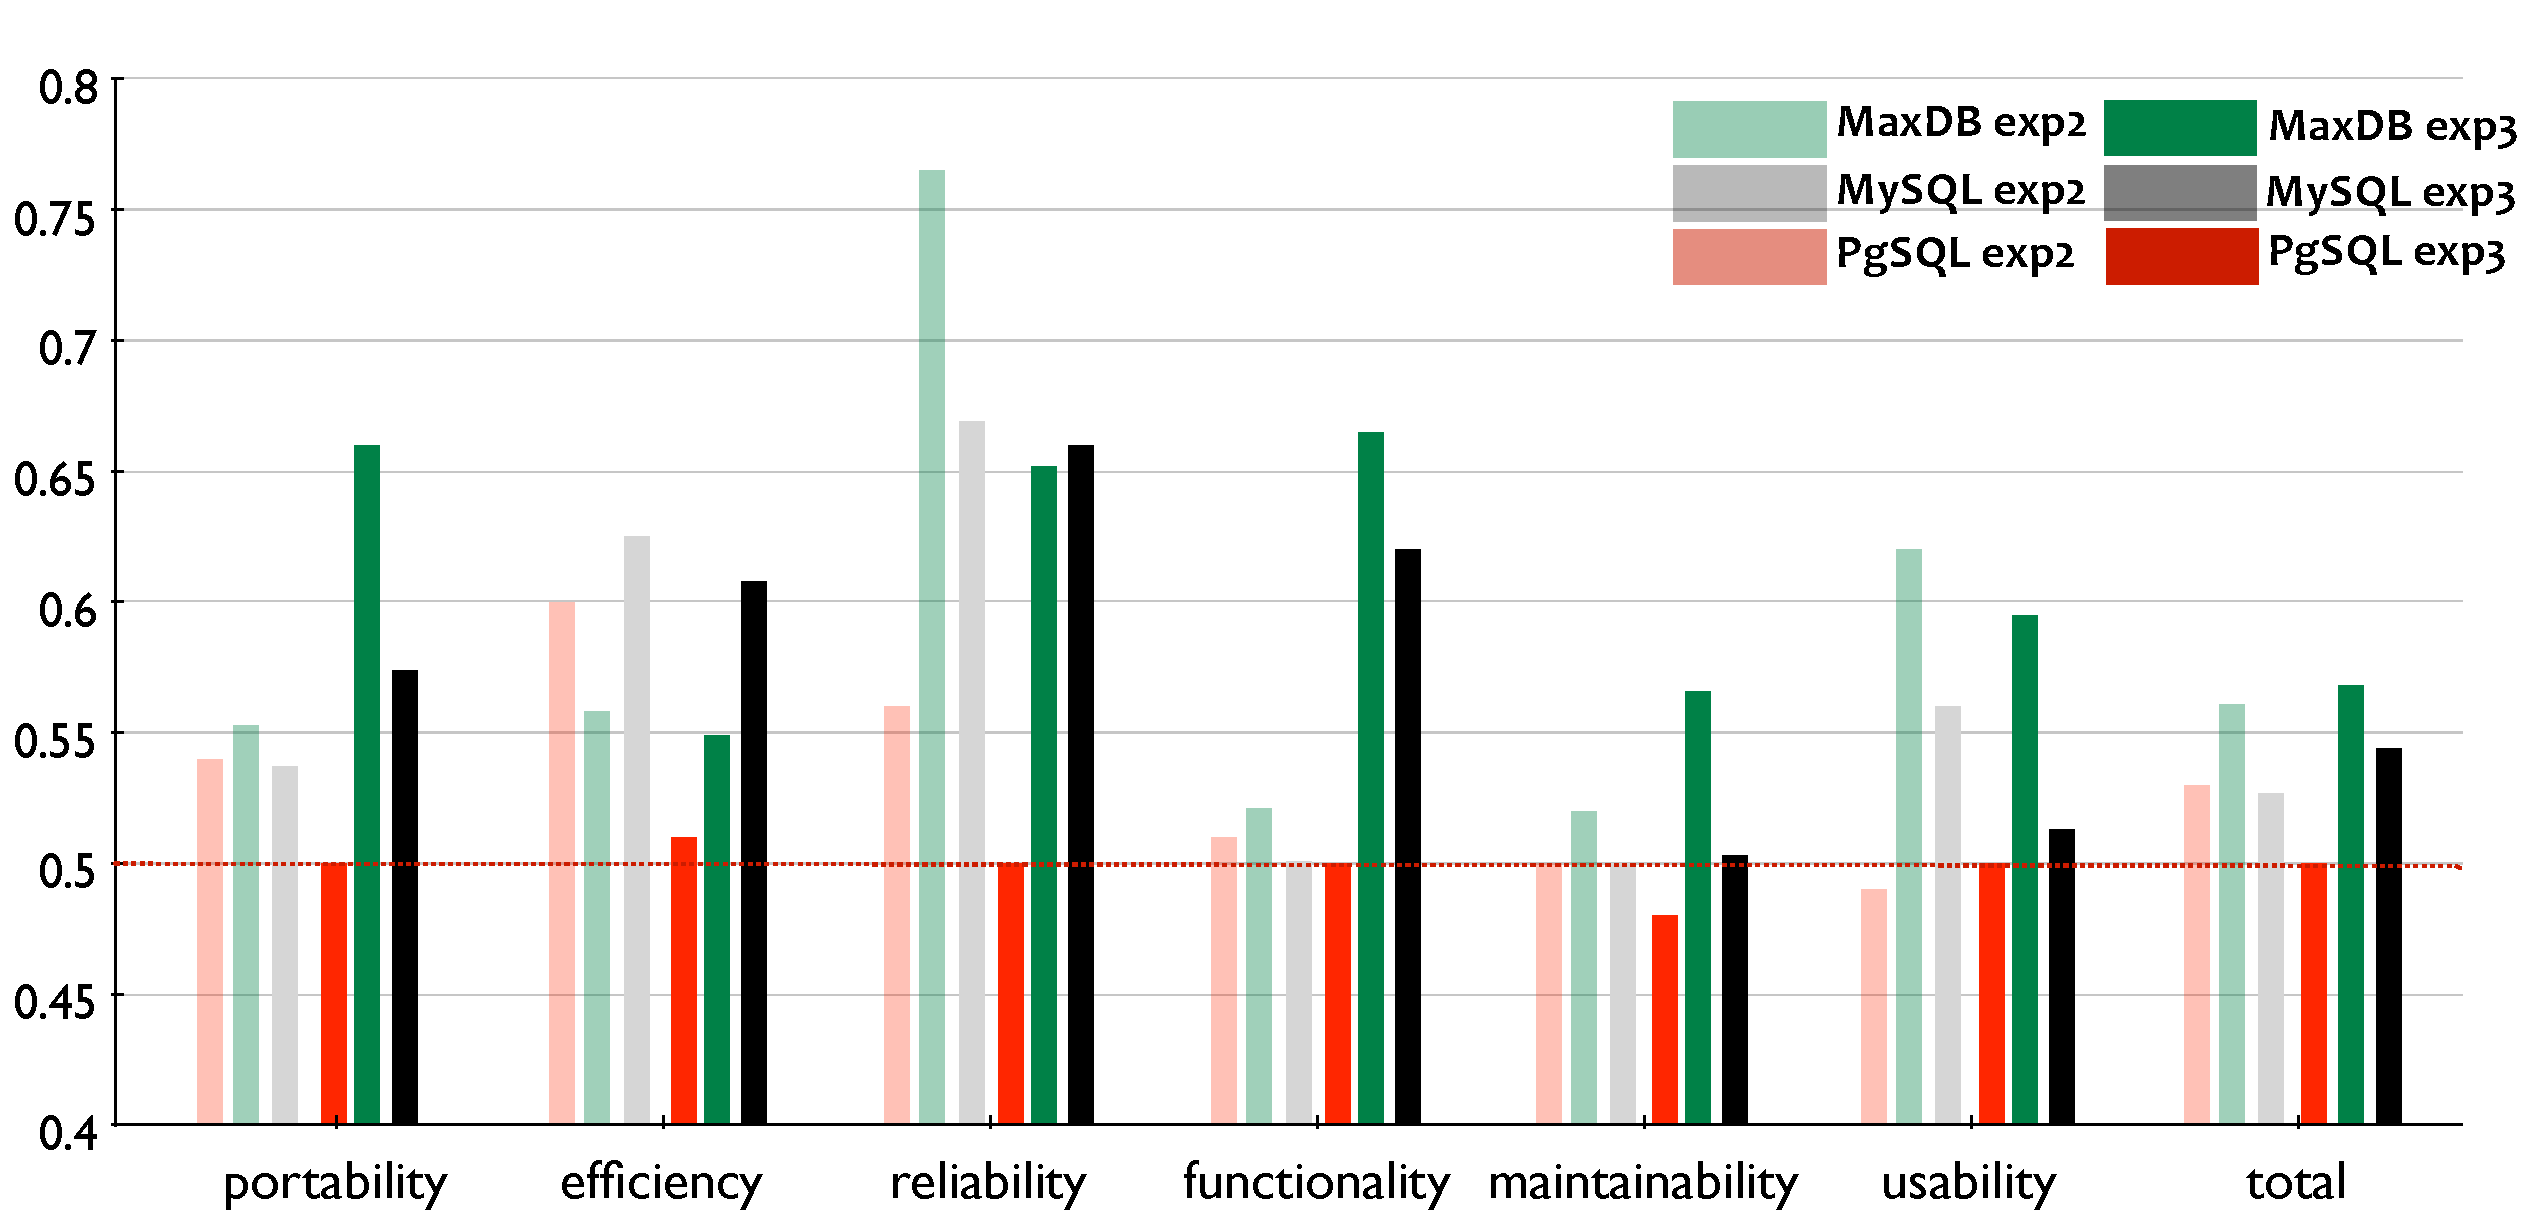
\includegraphics[width=0.45\textwidth]{figures/unsupervised-bar}
% \label{fig:maxdb-unsup-results-roc}
% }
% %\subfloat[F1]{
% %\includegraphics[width=0.45\textwidth]{figures/unsupervised-bar-f1}
% %\label{fig:maxdb-unsup-results-f1}
% %}
% \caption[]{Performance of unsupervised topic labelling for each NFR per word-list. A) ROC values -- 
% dashed line indicates the performance of a random classifier. B) F1 measure. Possible values range from 0--1.

% }
% \label{fig:maxdb-unsup-results}
% \end{figure}


\begin{figure*}[t]
  \centering
 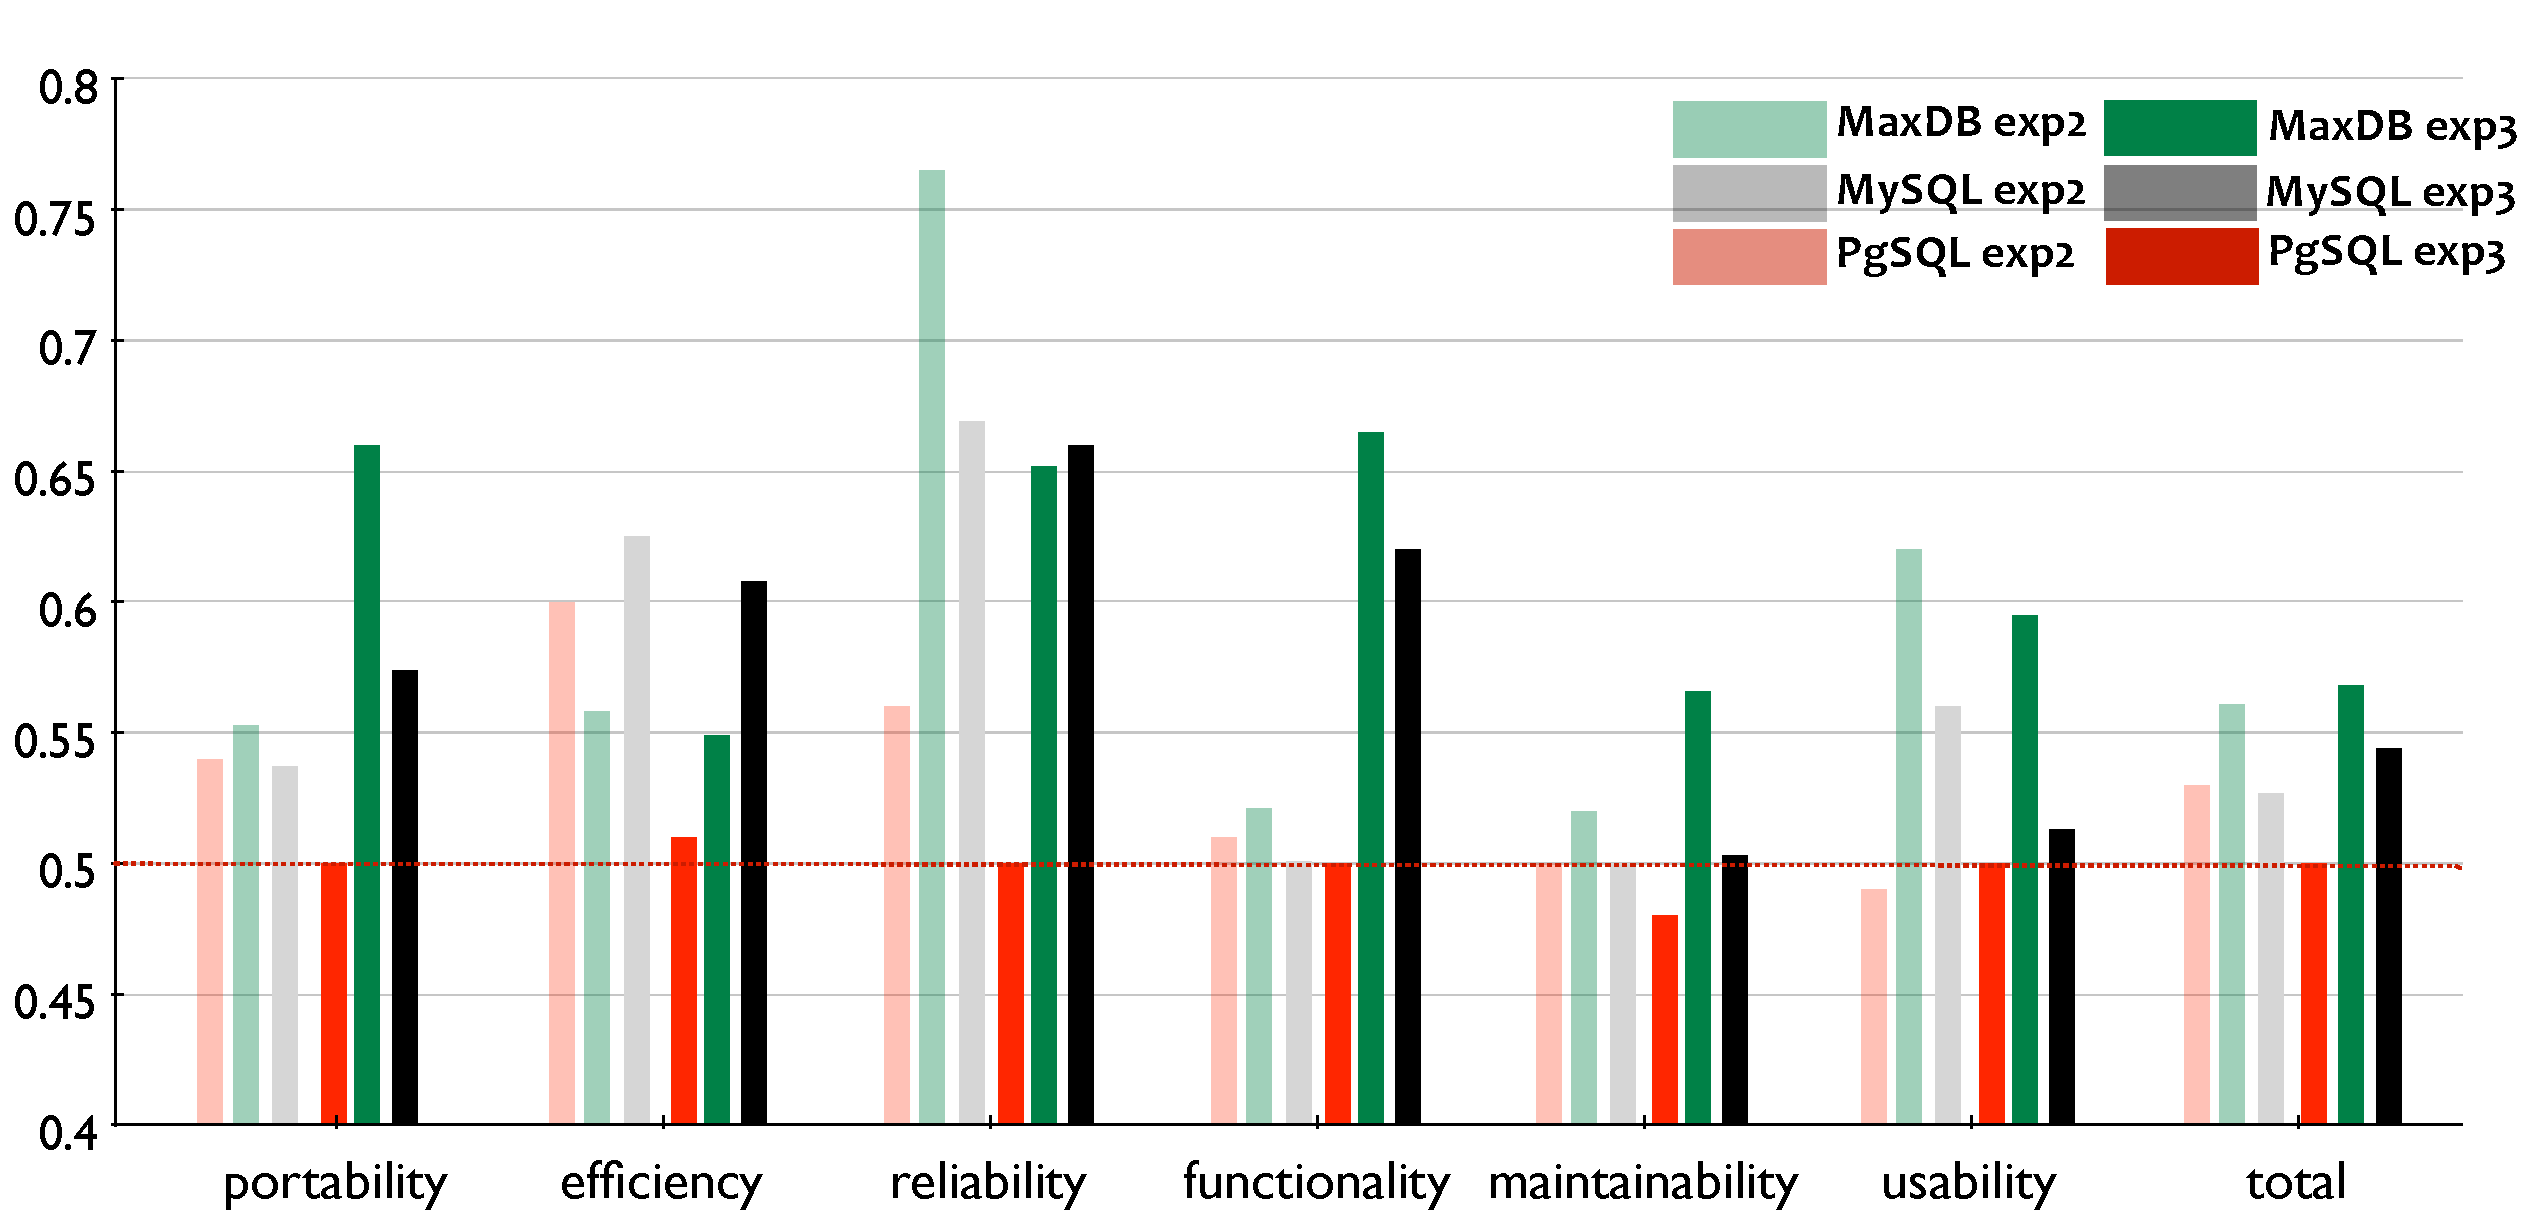
\includegraphics[width=0.9\textwidth]{figures/unsupervised-bar}
 \caption{Performance, ROC values (range: $0$--$1$), of semi-unsupervised topic labelling for
   each NFR and per word-list. The dashed line indicates the performance of a random classifier. This graph shows how well the
   semi-unsupervised topic labelling matched our manual annotations.}


  \label{fig:maxdb-unsup-results}
\end{figure*}


Because our ground truth annotations were relevant only to ISO9126,
 \textsf{exp1} had poor
performance due to the overlap between ISO9126 and the Kayed ontology (i.e., we annotated topics with labels which did not appear in the validation corpus). 
For \textsf{exp1} the F-measures for the NFRs for MaxDB were from $0$ to $0.18$ with an average (of all NFRs)
of $0.03$, for MySQL were from $0$ to $0.16$ with an average of
$0.05$, and for PostgreSQL $0$ to $0.15$ with an average of $0.07$. 

%\DONE{update these numbers but from where? }
% 0.177215189873 / 6
% .02953586497883333333
% (0.0298507462687 + 0.0661157024793 + 0.0634920634921 + 0 + 0.115384615385) / 6
% .04580718793751666666

% pgsql
% portability 
% 0.0910746812386
% efficiency 
% 0.154639175258
% reliability
% 0.0470588235294
% maintainability
% 0
% usability
% 0.0720720720721
%> v <- c(0.0910746812386 , 0.154639175258 , 0.0470588235294 , 0 , 0.0720720720721)
%> summary(v)
%   Min. 1st Qu.  Median    Mean 3rd Qu.    Max. 
%0.00000 0.04706 0.07207 0.07297 0.09107 0.15460 


% EXP2 source is latest-reports/exp2-unsup-results.xls. Numbers reflect latest runs as of 08/2011.
% (change as needed). Second column (after the name) is F1.
% column format is determined by info-theory.py : accuracy	f1	fn	fp	mcc	precisions	recall	roca	tn	tnr	tp
For \textsf{exp2}, the average F-measure (macro-F1) for MaxDB was  $0.24$ with a range $0.091$ to
$0.37$, and $0.16$ for MySQL with a range of $0$ to $0.41$. PostgreSQL had an average F-measure of $0.30$ %using pgsqln
 with a range of $0.09$ to $0.38$.
MaxDB had an average precision and recall of $0.25$ and $0.22$
while MySQL had $0.41$ and $0.10$ and PostgreSQL $0.31$ and $0.29$, respectively.

% EXP3
For \textsf{exp3}, the average F-measure (macro-F1) for MaxDB was $0.26$ with a range $0.11$ to
$0.47$, and $0.36$ for MySQL with a range of $0.10$ to $0.65$. 
PostgreSQL had an average of $0.42$ with a range of $0.31$ to $0.54$.
MaxDB had an average precision and recall of $0.16$ and $0.67$
while MySQL had $0.3$ and $0.48$. PostgreSQL had average precision and recall of $0.27$ and $0.95$, respectively.

Based on this we found that \emph{reliability} and
\emph{usability} worked well for MaxDB in \textsf{exp2} and better in
\textsf{exp3}. 
\textsf{exp1} performed poorly.
MySQL had reasonable results within \textsf{exp2} for \emph{reliability} and \emph{efficiency}. 
MySQL's results for \emph{efficiency} did not improve in \textsf{exp3}
but other qualities such as \emph{functionality} did improve. 
For PostgreSQL in \textsf{exp2}, \emph{reliability} and \emph{efficiency} were likewise the most accurate,
while \emph{functionality} remained poor. \emph{Functionality} improved dramatically by \textsf{exp3}.
Our F-measure scores were low and many ROC scores were $0.6$ or less, but our classifier, in most cases,
still performed substantially better than random ($0.5$), even in the
face of heavy class-imbalance for qualities such as \emph{usability} 
and \emph{efficiency}. While there is much room for improvement, we are seeing some
correlation between our quality word lists and relevant topics.

%\vspace*{-1em}
\subsection{Supervised Labelling}
\label{sec:suplabelling}
Supervised labelling requires expert analysis of the correct
class/label to assign a label to a topic. In our approach, we use the top-level NFRs in the ISO9126 standard~\cite{iso9126} for our classes, but other
taxonomies are also applicable.%In order to validate how effective these word-bag approaches to topic labelling would be we created a validation data set. 

We used a suite of supervised classifiers, WEKA~\cite{weka09},
that includes machine learning tools such as support vector machines and Bayes-nets. 
We also used the multi-labelling add-on for WEKA, Mulan~\cite{mulan}. %\footnote{\url{http://mlkd.csd.auth.gr/multilabel.html}}. 
Traditional classifiers label topics with a single class, whereas Mulan allows for a mixture of classes per topic, which is what we observed while
manually labelling topics. For example, a given topic (word distribution) may be `about' both usability and maintainability, if this topic was a product of a discussion on design tradeoffs.
The \emph{features} we used are word counts/occurrence	per topic, if
a word occurs frequently enough in a topic we consider it a feature of
the topic.

To assess the performance of the supervised learners, we did a 10-fold cross-validation~\cite{Kohavi1995}, a common technique for evaluating machine
learners. 
The original data is partitioned randomly into ten sub-samples. Each sample is used to test against a training set composed of the nine other samples.
%One subsample is used as a training set and evaluated on the other nine sub-samples. 
%This is repeated nine more times, with each subsample used once as the training set. 
We have reported these results below.% in Section \ref{sec:suplabelling}.

\subsubsection{Analysis of the Supervised Labelling}
% \label{sec:suplabelling}
Because our data-set was of word counts we expected Bayesian techniques, often used in spam filtering, to perform well. 
We tried other learners that WEKA~\cite{weka09} provides: rule learners, decision tree learners, vector space learners, and support vector machines.  
Figure \ref{fig:best-learn-per-tag} shows the performance of the best
performing learner per label: 
% We considered the best learner for a label to be 
the learner that had the highest ROC value for that label. 
The best learner is important because one uses a single learner per
label. When applying our technique, for each NFR one should select the
best performing learner possible. Given the tractability of these techniques, a tool which applied all learners and presented the best result should be feasible. 
%Figure \ref{fig:best-learn-per-tag} uses the ZeroR learner as a baseline, a common practice in machine learning,
%as ZeroR naively chooses the largest category all of the time. 
%ZeroR occasionally outperforms other learners; for labels which are not as common, this is to be expected because any miscategorization will hurt accuracy. 
%This is why we use ROC values, instead of accuracy, as they can better represent performance on labels which are not applicable to the majority of samples.

Figure \ref{fig:best-learn-per-tag} shows that MaxDB and MySQL have
quite different results, as the ROC values for \emph{reliability} and
\emph{functionality} swap between projects. For PostgreSQL, the
performance is nearly always poorer than the other two systems. The
reason for this lack of performance could be that parameter we chose for number of
topics, $N$, could be non-optimal for PostgreSQL. One explanation is that given the size of the PostgreSQL dataset, it was becoming hard to distinguish one topic
from the next. PostgreSQL's data-set was the largest of the 3 projects:
the XML datafile that described the PostgreSQL topics that we
annotated was 8 times larger than MySQL and 1.7 times larger than MaxDB. These
size differences arise from the number of commits, the number of files
and the verbosity of the commit descriptions.

%\DONE{expand on why?}

% PG data from abram's email of 09/01/2011 using first column and pgsqln.
\begin{figure}[t]
\centering
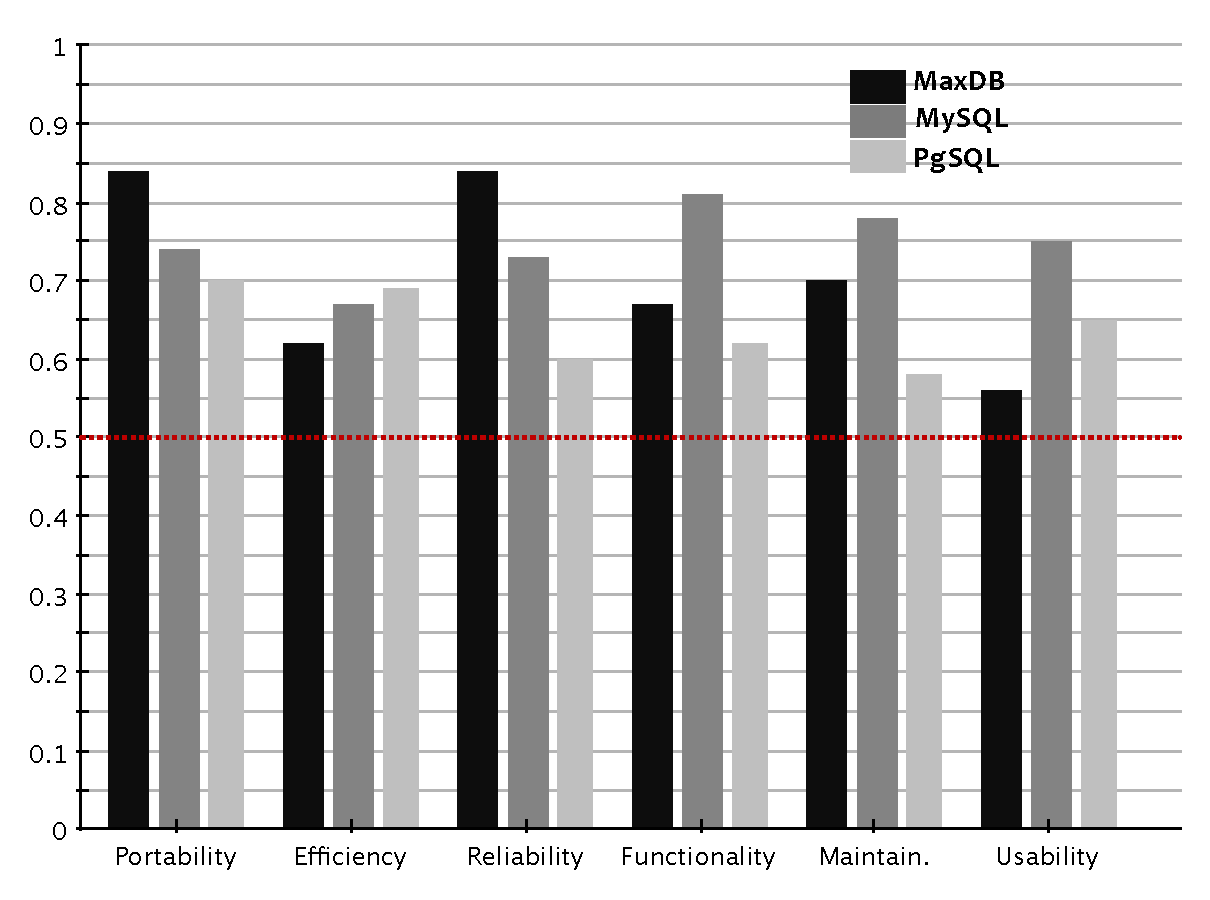
\includegraphics[width=0.7\textwidth]{figures/both-supervised}
\caption[]{ROC value for the best learner per label for MaxDB, MySQL and PgSQL. Values range from $0$--$1$.  Dashed line indicates the performance of a random
classifier.
}
\label{fig:best-learn-per-tag}
\end{figure}

For all projects Bayesian techniques did the best out of a wide variety of machine learners tested, due to the large number of features they can handle.
Our best learners, Discriminative Multinomial Naive Bayes, Naive Bayes
and Multinomial Naive Bayes  are all based on Bayes' theorem and all
assume, naively, that the features supplied are independent. 
%The features we used are word counts per message. 
One beneficial aspect of this result is that it suggests we can have
very fast training and classifying  since training on or classifying one
instance with Naive Bayes can be calculated in $O(N)$
for $N$ features.
%http://nlp.stanford.edu/IR-book/html/htmledition/naive-bayes-text-classification-1.html

% # F measure
% mysql
% > v <- c( 0.64 , 0.23  ,0.41 , 0.77  ,0.62 , 0.21 ) 
% > summary(v)
%    Min. 1st Qu.  Median    Mean 3rd Qu.    Max. 
%   0.210   0.275   0.515   0.480   0.635   0.770 
% maxdb
% > v <- c(0.61, 0.25, 0.59, 0.32, 0.42, 0.17)
% > summary(v)
%    Min. 1st Qu.  Median    Mean 3rd Qu.    Max. 
%  0.1700  0.2675  0.3700  0.3933  0.5475  0.6100 

%src/validate/latex-out/best-learner-per-project-roc
The range of F-measures for MySQL was $0.21$ to $0.77$ with a mean
of $0.48$. MaxDB had a range of $0.17$ to $0.61$ with a mean
of $0.39$. Finally, PostgreSQL had a range of $0.04$ to $0.9$ and a mean of $0.43$.


The less-frequently occurring a label, the harder it is to get accurate
results, due to the high noise level. Nevertheless, these results are
better than our previous word-list results of \textsf{exp2} and
\textsf{exp3}, because the ROC values are sufficiently higher in most
cases (other than MaxDB \emph{reliability}, MySQL \emph{efficiency}, and PostgreSQL \emph{maintainability}). The
limitation of the approach we took here is that we assume labels are
independent; however, labels could be correlated with each other. 
The next section (\ref{sec:multilabel})
addresses the issue of a lack of independence and correlation between
labels
using multi-label learners.
%In the next section we will evaluate how well these learners perform
%together.
%\DONE[inline]{Comment about correlation, we should link to the Mulan section, perfect segway since Mulan relies on correlation.}

%\balance

\subsection{Applying Multiple Labels to Topics}
\label{sec:multilabel}

As noted in Section \ref{sec:wordlist}, each topic in our data-set can be composed of zero or more NFRs. 
For example, a commit message might address \textit{reliability} in the context of \textit{efficiency}, or make a \textit{maintainability} improvement
in the source code that related to \textit{usability}. 
However, traditional machine learning techniques, such as Naive Bayes, can only map topics to a single class. 
The Mulan~\cite{mulan} library encapsulates several different multi-label machine learners which can label elements with multiple labels.
Mulan also includes methods for determining the performance of these learners.
% TOO DETAILED The problem framed in the learners above has changed; instead of looking at the precision and recall of applying one label, we rank
% multiple labels at once. We must check if the full subset of labels was applied, and then how much of that subset was applied.

% Data source is src/validate/output/<db>.mulan.out.tex
% pgsqln & br & clr & homer
% macro-auc .64 .58 .58
% micro .65 .6 .6
%pgsqla
% macro .63 .56 .54
% micro .81 .81 .79
% maxdb (no macro)
% micro .77 .67 .61
% mysql
% macro .74 .65 .64
% micro .81 .8 .74

\begin{figure*}[t]
\centering
\subfloat[MySQL]{
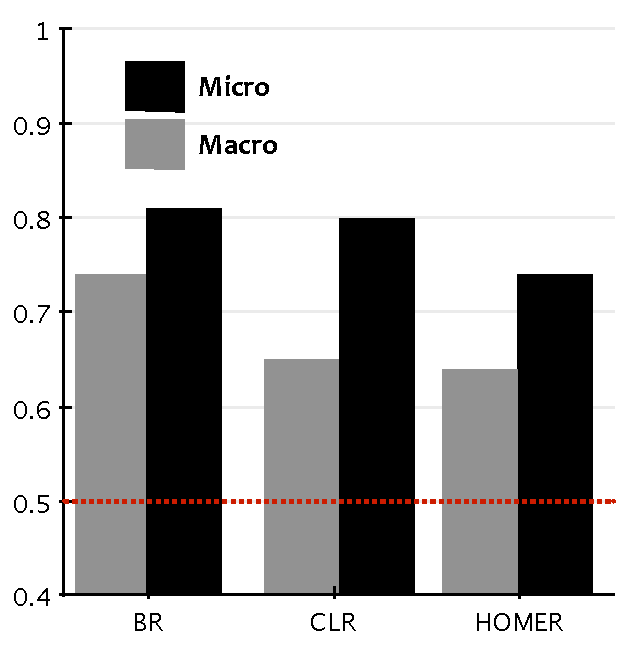
\includegraphics[width=0.4\textwidth]{figures/multi-label-results-mysql}
\label{fig:subfig3}
}
\subfloat[MaxDB]{
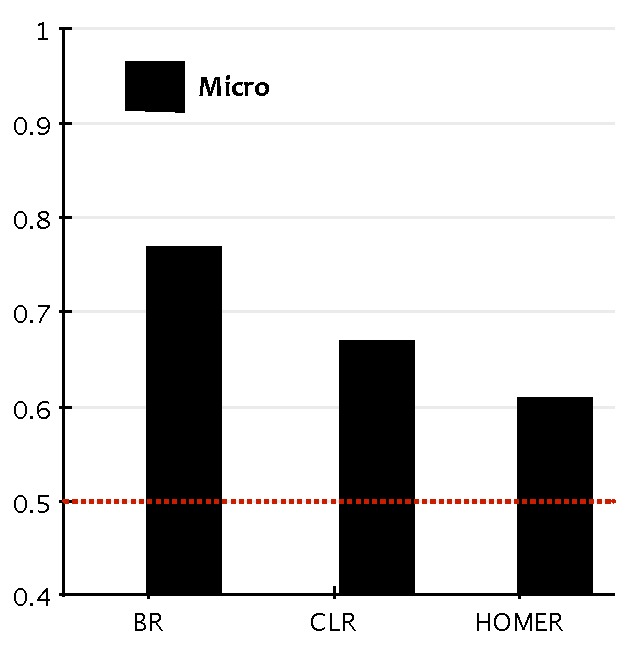
\includegraphics[width=0.4\textwidth]{figures/multi-label-results-maxdb}
\label{fig:subfig4}
}
\caption[]{MySQL and MaxDB macro and micro-ROC results per multi-label learner. Possible values range from $0$--$1$.  Dashed line indicates the performance of a random classifier.
}
\label{fig:mulan}
\end{figure*}

\begin{figure}
\centering
\subfloat[Macro-ROC]{
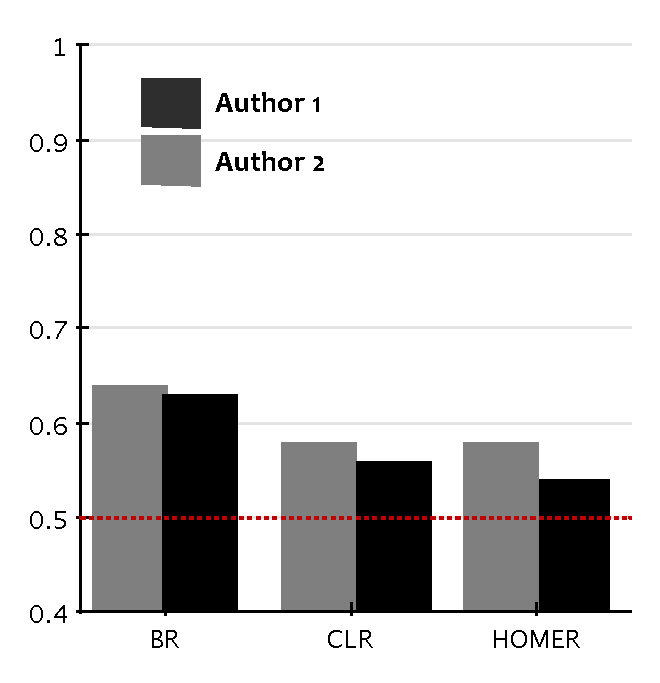
\includegraphics[width=0.4\textwidth]{figures/pg-mulan-macro-compare}
\label{fig:pgcomp-a}
}
\subfloat[Micro-ROC]{
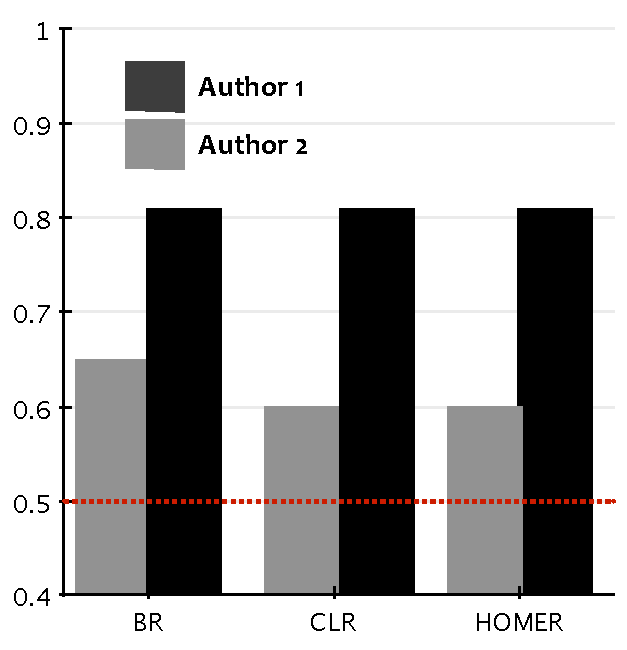
\includegraphics[width=0.4\textwidth]{figures/pg-mulan-micro-compare}
\label{fig:pgcomp-b}
}
\caption{Author \#1 and author \#2 ROC results for PostgreSQL.} 
\label{fig:pgcomp}
\end{figure}

Two perspectives used to evaluate multi-label learners are with micro or macro measurements (shown in Figure \ref{fig:mulan}a).
Macro measurements are aggregated at a class or label level (per class) while micro measurements are at the element level (per element).
A macro-ROC measurement is the average ROC over the ROC values for all labels, where a micro-ROC is the average ROC over all examples that were classified. 
For MaxDB, the macro-ROC values are undefined because of poor performance of one of the labels.%, see Figure \ref{fig:mulan}.

Figure~\ref{fig:mulan} presents the results of Mulan's best multi-label learners for the MaxDB and MySQL projects, and  Figure~\ref{fig:pgcomp} for PostgreSQL. 
Calibrated Label Ranking (CLR) is a learner that builds two layers. The first layer determines if an entity should be labelled, while the second layer
determines what labels should be assigned.
The Hierarchy Of Multi-label classifiERs (HOMER) and Binary Relevance (BR) act as a hierarchy of learners: BR is flat, while HOMER tries to build a
deeper hierarchy for a more accurate learner~\cite{mulan}. 

Figure~\ref{fig:pgcomp} shows the ROC results for the PostgreSQL
product. In this figure, we show the relative differences when we use
different training data sets from different annotators. In \ref{fig:pgcomp-a} we see that ROC
results are very similar. In the other figure, however, author \#1 has
dramatically better performance. We speculate that this is due to the
particular annotation decisions made by author \#1; in some sense he
performed better. 
The difference in Macro-ROC was not significant, but the difference in
Micro-ROC was, as the p-value of Student's T-test was $< 0.001$. 
%\DONE{check this writeup of comparison. T-test useful}

These classifiers performed better than other multi-label classifiers as they have the best micro and macro ROC scores. 
The multi-label and single-label learners had similar performance: for
MySQL, BR and Naive Bayes had similar macro-ROC scores of $0.74$.

\section{Understanding Software Maintenance Activities} 
\label{sec:analysis}
As we mentioned in the introduction, a key issue in software maintenance is understanding \emph{why} a system has evolved the way it has~\cite{aranda09icse}. 
In this section we demonstrate the value of labelled topic extraction
in addressing this issue. 
% more why
Labelled topics address \emph{why}  because they show reasons why changes
occurred rather than \emph{how}. 
The \emph{how} of a change is the change itself, the purpose or
\emph{why} is what we are after.
We investigate the history of the three large-scale database systems that we studied. 
We use our technique to show the topic of development efforts over time in each project.
%We evaluated two research questions using the ground truth data that we annotated by hand:
We motivated our investigation with three research questions:
\begin{enumerate}
\item \emph{Do NFR frequencies change over time?} If a particular NFR
  was of more interest at one point in the life-cycle than another,
  this suggests that development activity shifted focus. For example,
  if a developer expected to see a recent focus on \emph{reliability},
  but instead \emph{usability} dominated, they might re-prioritize
  upcoming work items.

\item \emph{Do projects differ in their relative interest in NFRs?} A
  project manager, especially a systems-manager, would be interested
  in knowing whether a particular NFR, such as \emph{reliability}, was
  more important for one project than another. This question could be used to
  confirm the initial design goals, or to track the progress on that
  quarter's objectives.  The difference in NFR proportion is
  interesting because it implies a difference in focus between projects.

\item \emph{Do different developers work on different NFRs?} For a given project, it is reasonable to think that developers are either assigned
(in commercial organizations) or choose (in open-source organizations) to work on a particular NFR. For example, one developer might be more junior, and take
responsibility for the low-impact reliability fixes. Another, more senior developer might assume responsibility for major improvements such as efficiency
improvements. 

\end{enumerate}


%\subsection{Timeline analysis}
Topic time-lines are depicted in Figures \ref{fig:mysql-timeline}, 
\ref{fig:maxdb-timeline} and \ref{fig:pgsql-timeline}. These topic time-lines show the
temporal patterns of NFR frequencies.
%NEIL- I think this (below) is just confusing, although maybe important to note.
This is generated from the manually annotated
topics, although this visualization can be generated from the
results of labelled topic extraction. Note that there are no unlabelled topics in this dataset.

There are two measures represented. 
One, the relative frequency, shown in the grey histogram boxes, represents the number of topics with that NFR in that period, 
relative to the maximum number of topics assigned to the NFR. 
For example, in Figure \ref{fig:mysql-timeline} we see a spike in \emph{portability} and \emph{functionality} frequency in September 2002.
The second, absolute frequency, is shown using cell intensity, and compares the number of topics labelled with the NFR per period 
relative to the maximum number of labelled topics overall. 
For instance, Figure \ref{fig:mysql-timeline} shows that the NFRs
\emph{functionality}, \emph{portability} and \emph{maintainability}
contain more labelled topics, since these NFRs have been more
intensely shaded. One interesting stream is \emph{efficiency} in PostgreSQL, which shows periodic
activity, and suggests that efficiency-related changes
have longer lasting effects. A more systematic analysis of periodicity is necessary to properly conclude this.
The topmost row in each diagram lists historical events for that project (such as a release). 
%We refer to these occurrences in the discussion which follows.

\begin{figure}[t]
\centering
\subfloat[MySQL 3.23]{
%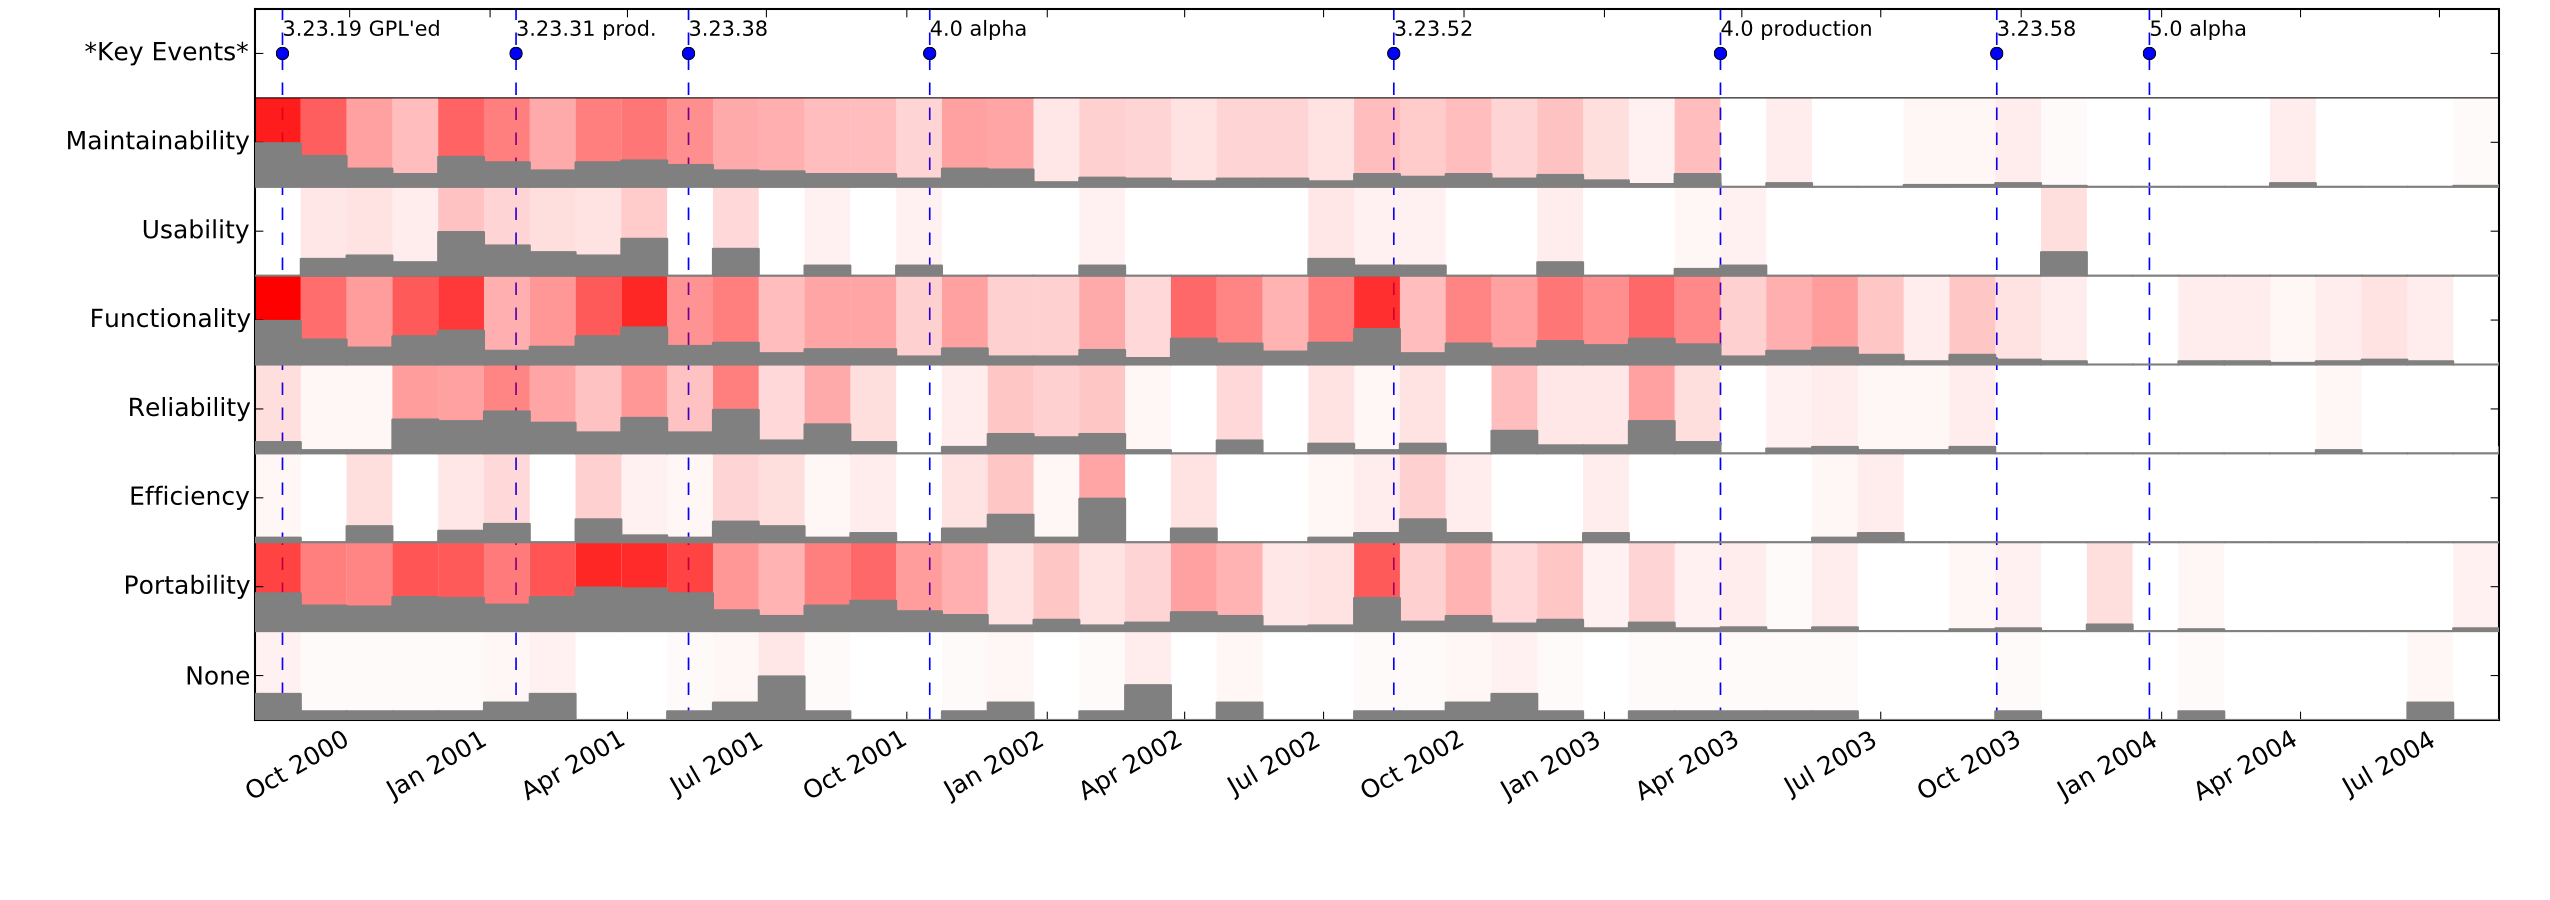
\includegraphics[width=\textwidth]{figures/mysql-timeline.png}
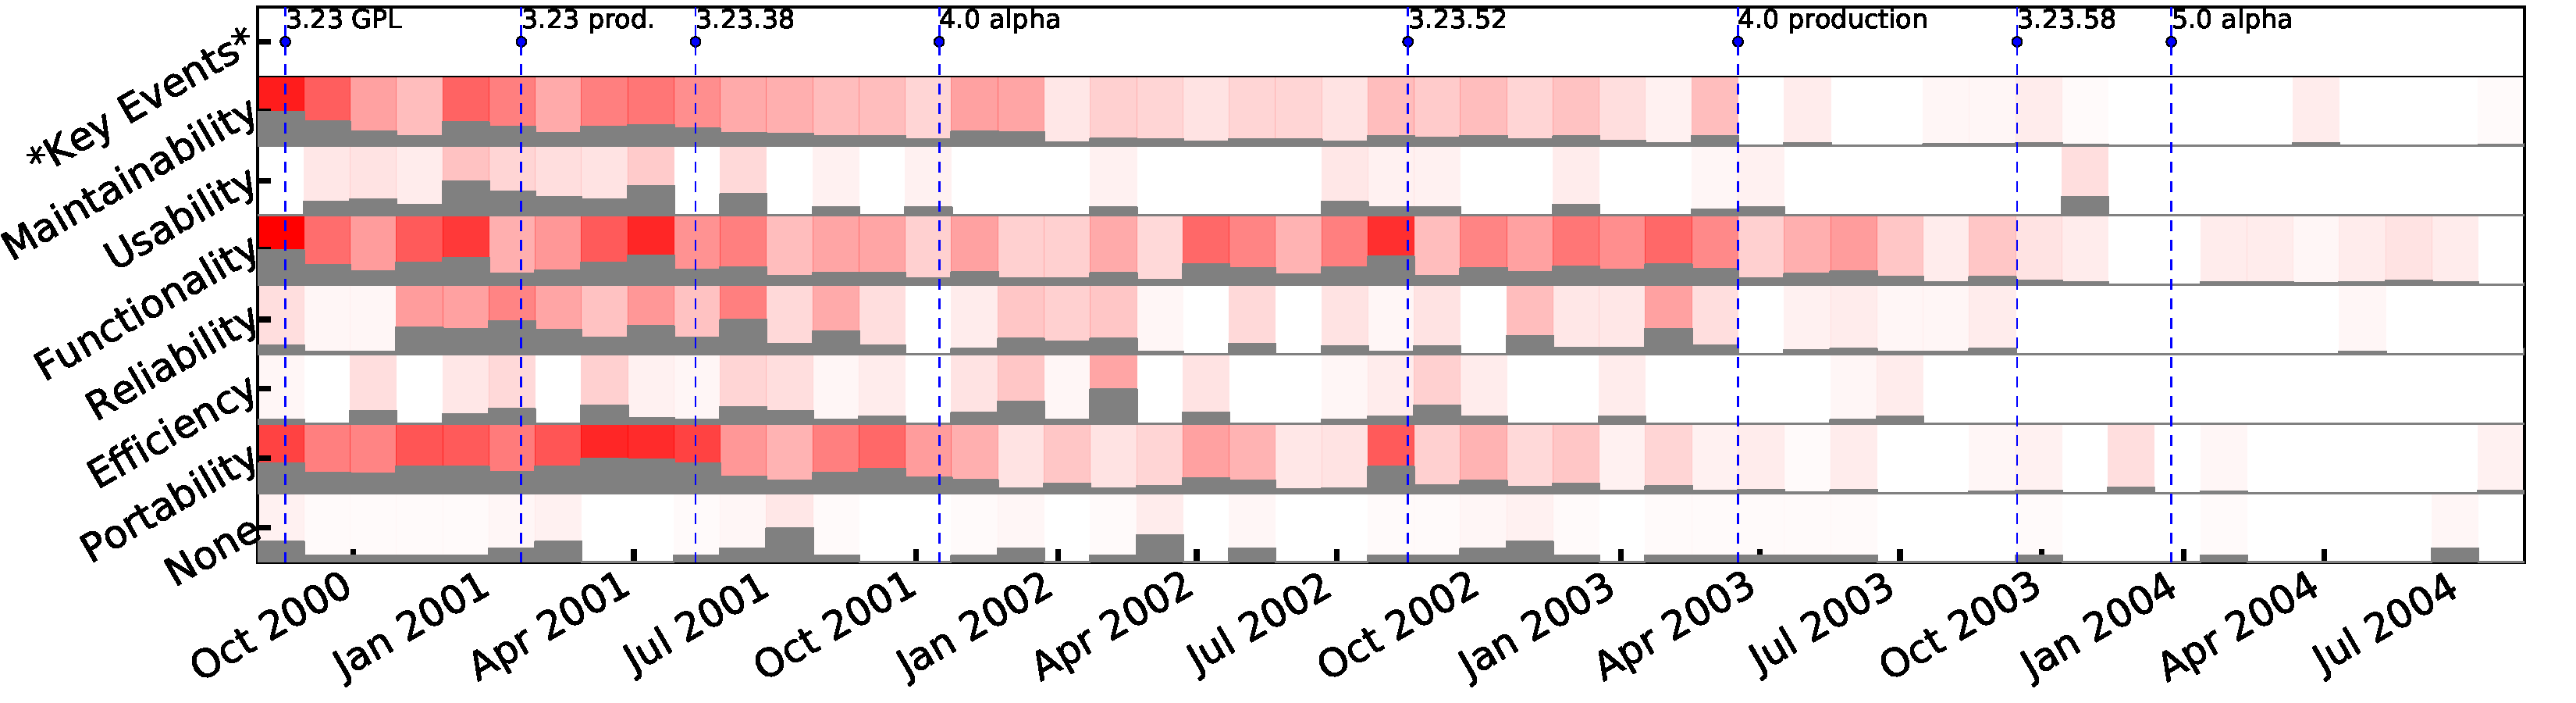
\includegraphics[width=\textwidth]{figures/mysql-timeline}
\label{fig:mysql-timeline}				 
}	    
					     
\subfloat[MaxDB 7.500]{					
%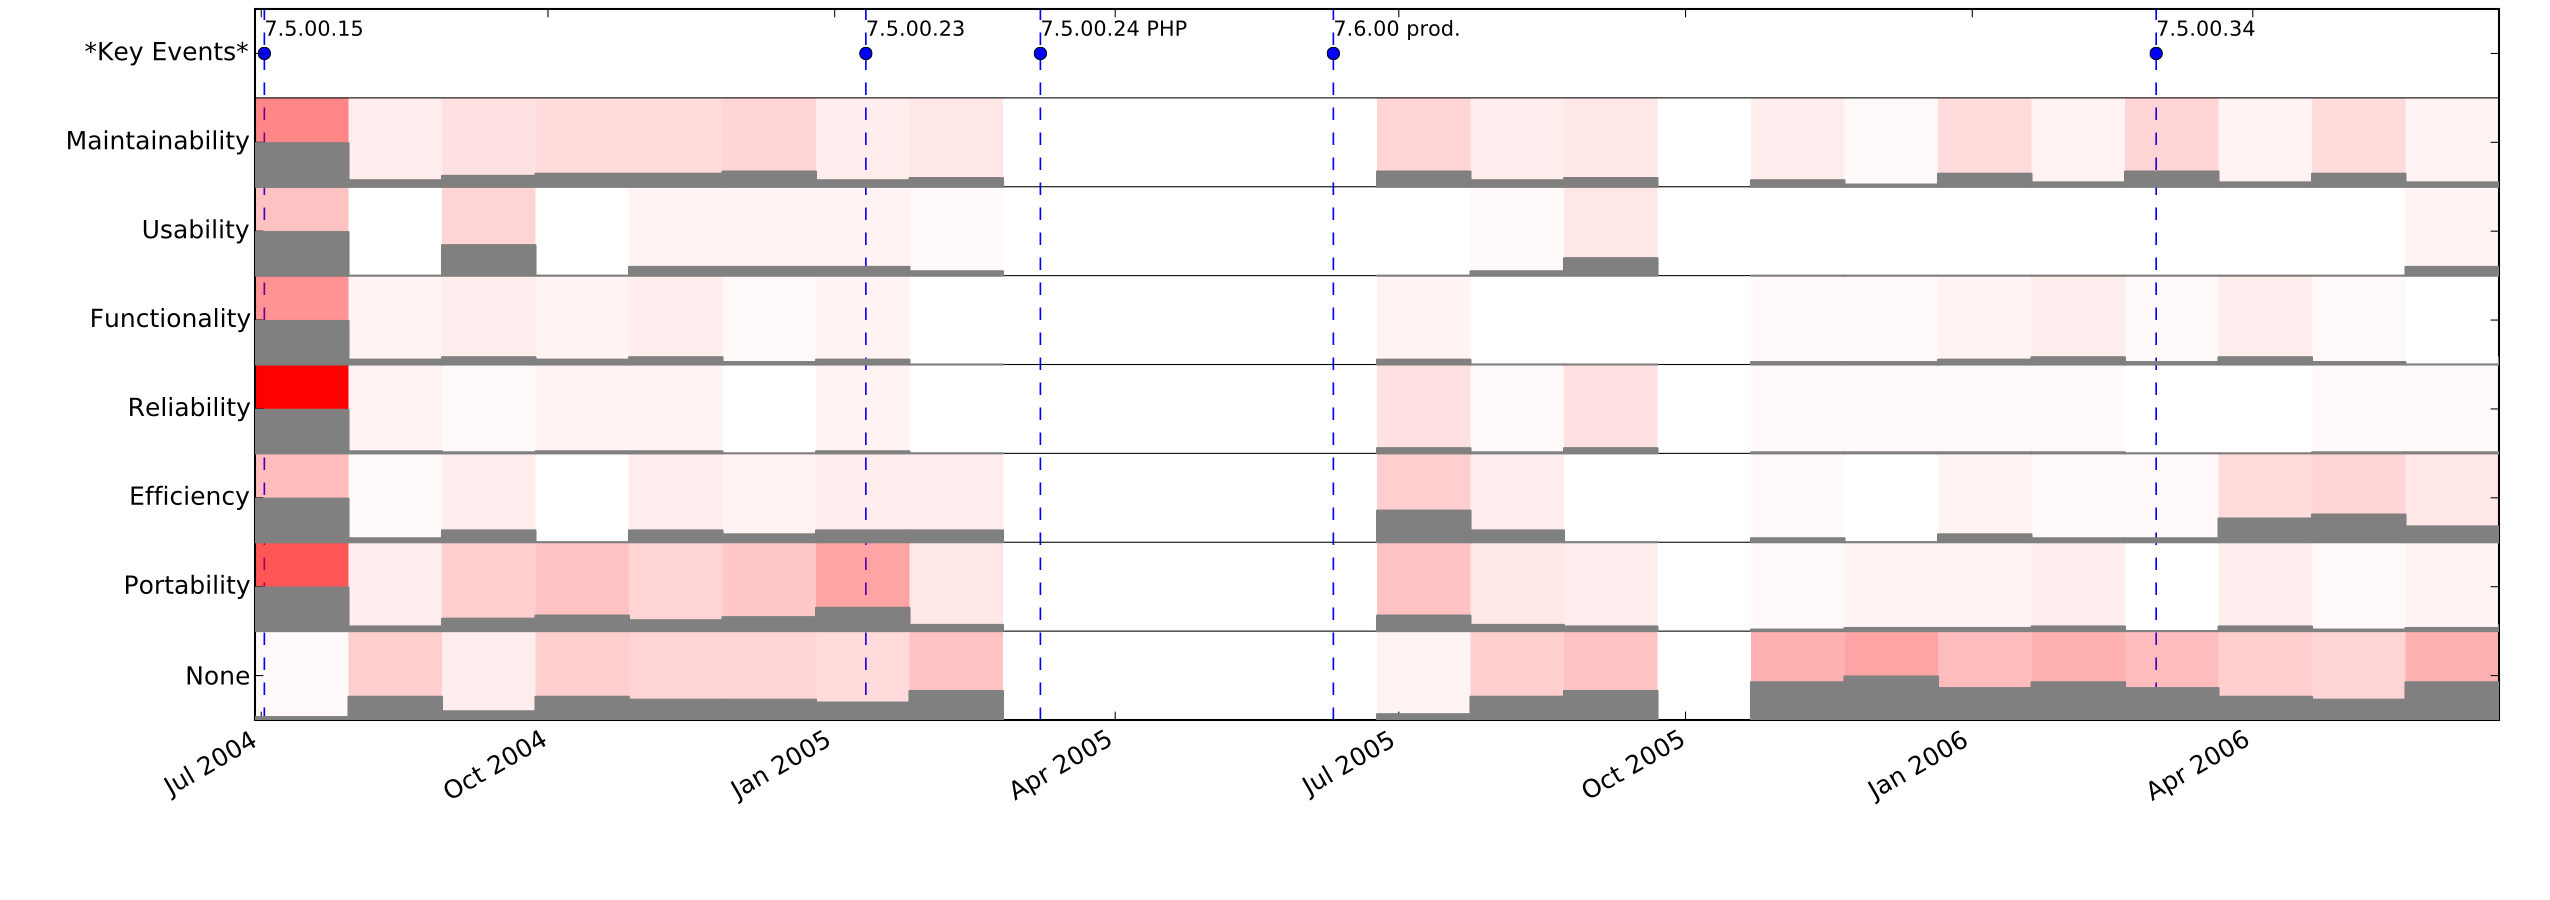
\includegraphics[width=\textwidth]{figures/maxdb-timeline.png}
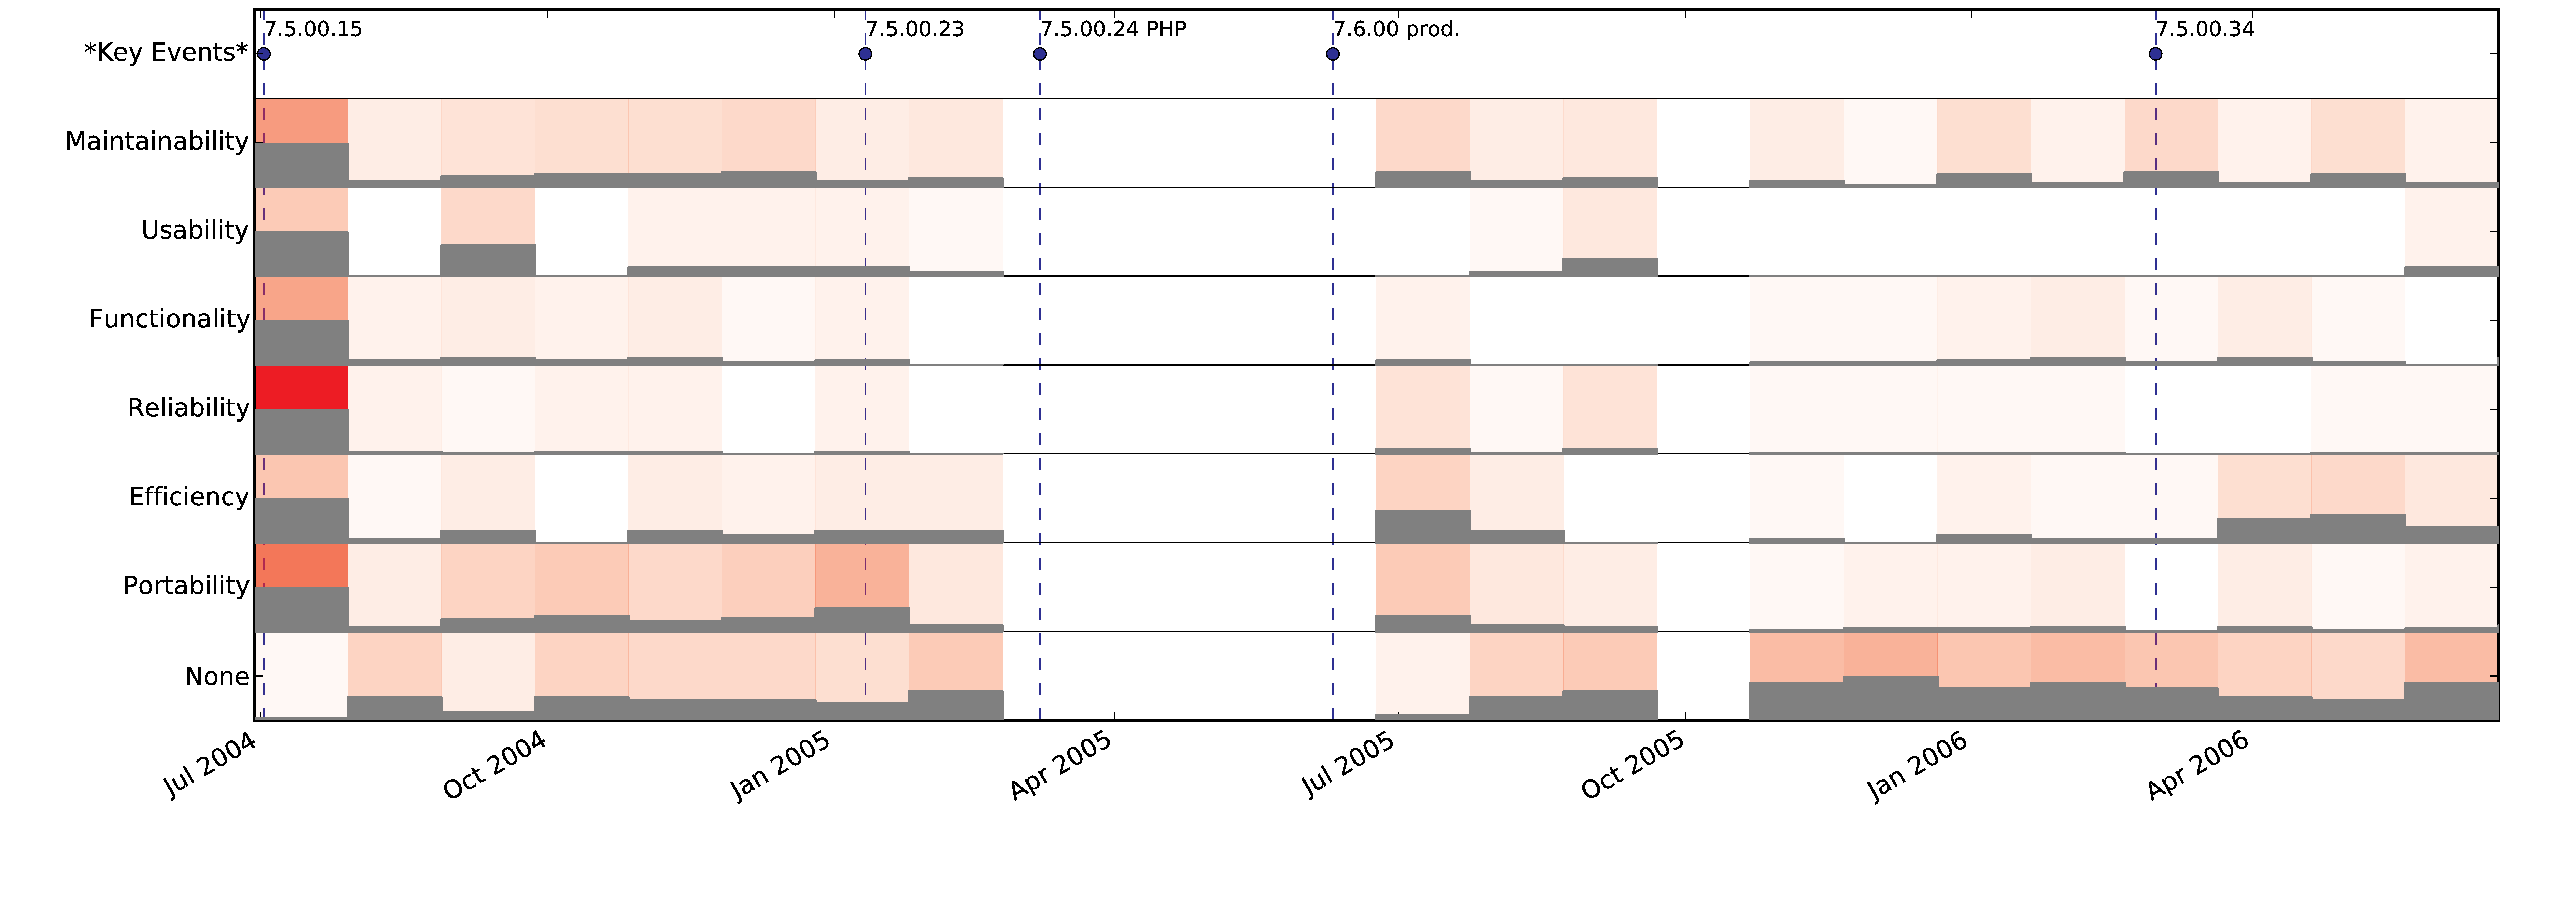
\includegraphics[width=\textwidth]{figures/maxdb-timeline}
\label{fig:maxdb-timeline}
}

\subfloat[PostgreSQL 7.2]{					
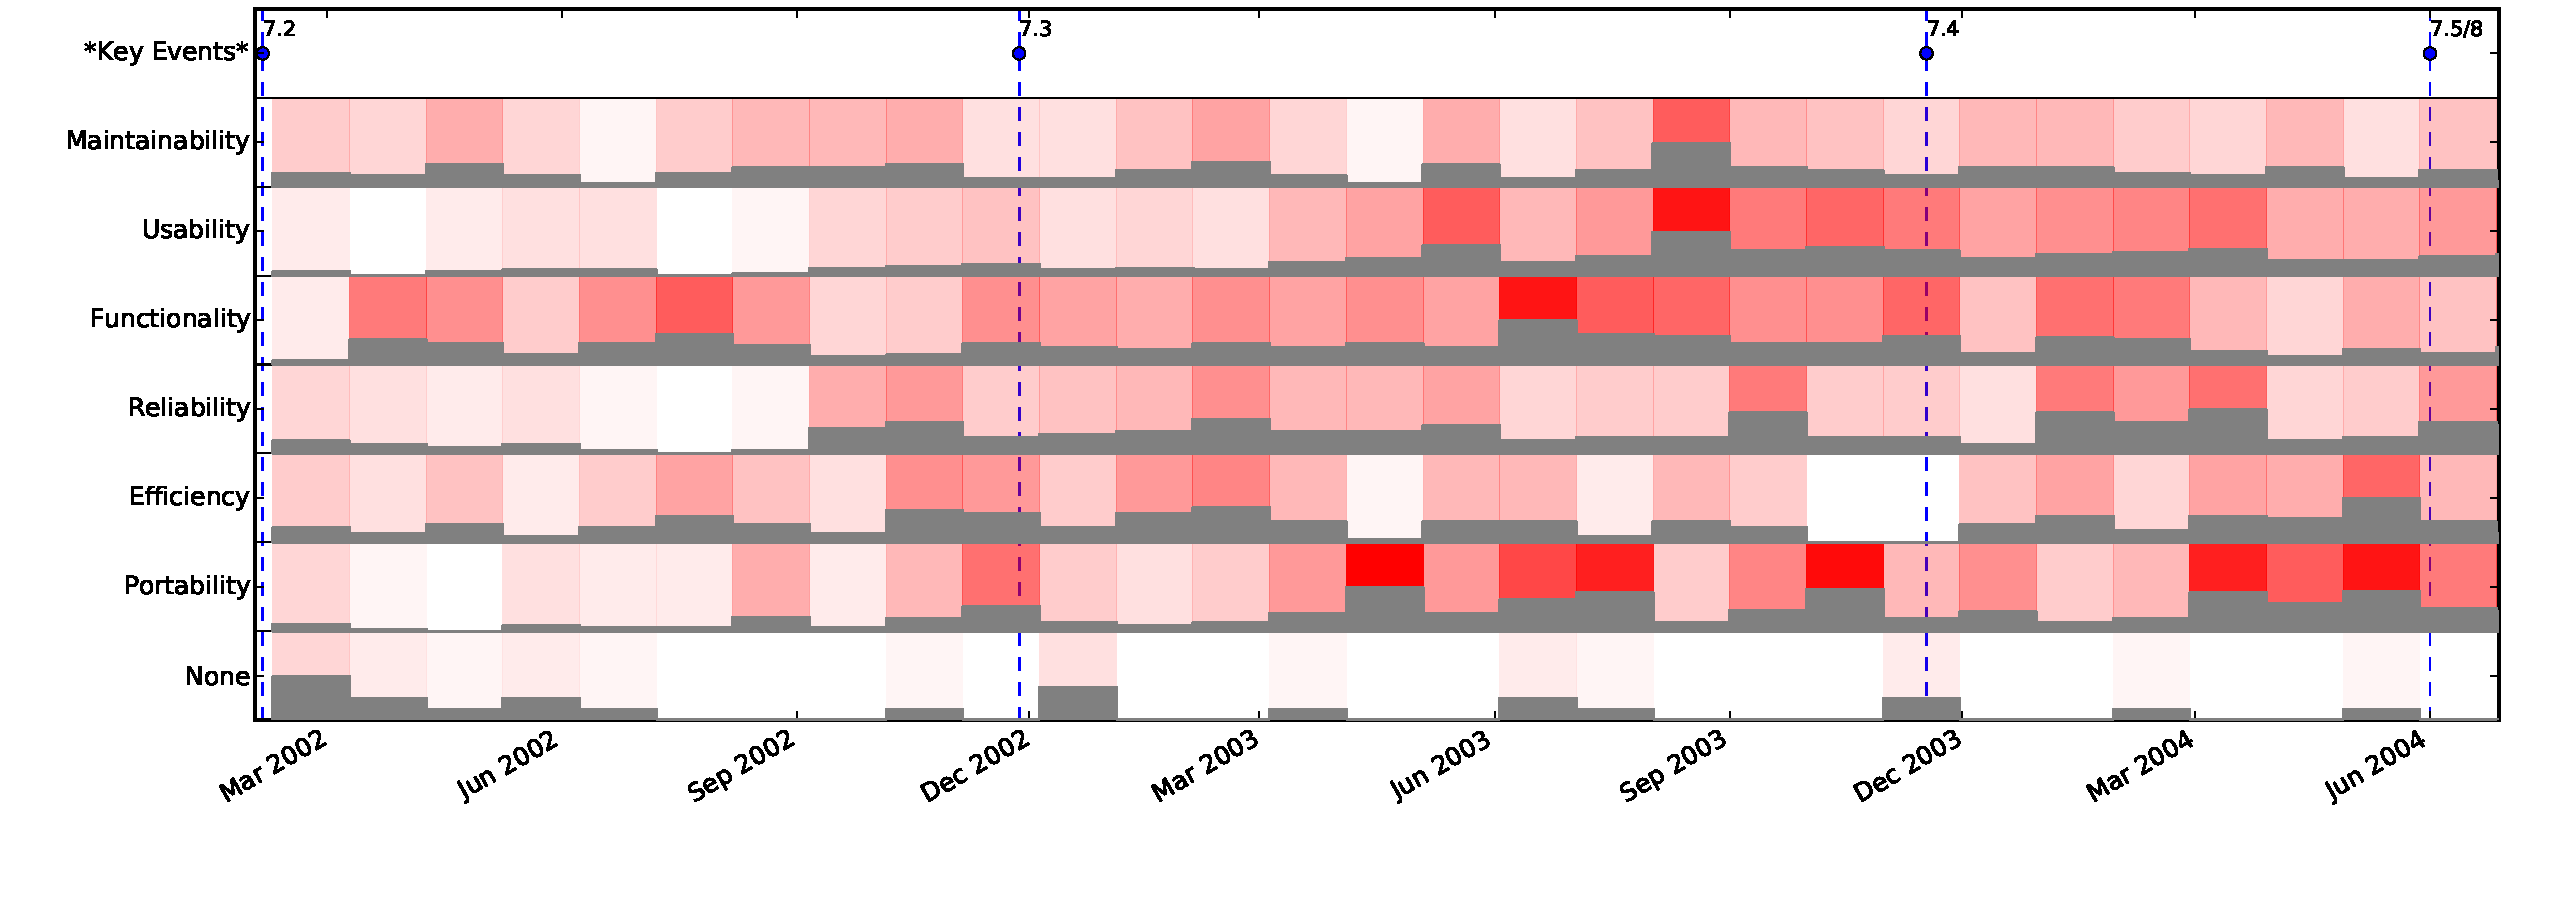
\includegraphics[width=\textwidth]{figures/pgsql-timeline}
\label{fig:pgsql-timeline}
}
	\caption[]{NFR label per period. Each cell represents a 30-day period. %Numbers represent number of topics in that period labelled with that NFR. 
	Grid cell intensity (saturation) is mapped to label frequency
	relative to the largest label count of \emph{all} NFRs. Grey
	histogram bars indicate label frequency relative to that
	particular NFR's largest label count. Dashed vertical lines
	relate a project milestone (\emph{*Key events*}) to our topic windows. 

}
\label{fig:timelines}
% Timelines created using src/validate/summary_labels.py
\end{figure}

%\noindent \textbf{Understanding the figures} -- 
 % boxes. not sure boxes is important..
% I grepped query1.mrs2 http://softwareprocess.es/y/y/maxdb-76.tar.gz
% and			http://softwareprocess.es/y/maxdb-7500.tar.gz
%There are more \textsf{None} labels in MaxDB because a number of topics were to do with code cleanup or automated checking using tools like
%\texttt{sutcheck}, a tool specific to the development process of MaxDB. 

%\noindent \textbf{Timeline of key events} -- 
We analyzed each project's developer mailing list for external validation (the body of the email).
%As discussed earlier, the top row in each figure shows key events for each project. 
We use \textit{labelled topic extraction} to pick out the underlying NFR activity behind these events. 
For example, both MaxDB and MySQL show a high number of NFRs recognized at the first period of analysis. 
This is due to our window choice: we deliberately targeted our
analysis to when both MySQL 3.23
and MaxDB 7.500 were first announced. For MaxDB, version 7.5.00  was released in December of 2003. 
We know that release 7.5.00.23 saw the development of PHP interfaces, possibly accounting for the simultaneous increase in the \emph{portability}
NFR at the same time.
The gap in MaxDB (Figure \ref{fig:maxdb-timeline}) is due to a shift in development focus (from February 2005 to June 2005) to MaxDB 7.6, which is
released in June 2005.

%For MySQL (Figure \ref{fig:mysql-timeline}), we similarly validated our NFR patterns with external mailing list data. 
The development period of MySQL we studied  (Figure \ref{fig:mysql-timeline}) saw the first releases to be licensed under the GPL. 
Version 3.23.31 (January, 2001) was the production release (non-beta), and the timeline view shows a flurry of topics labelled with \emph{functionality} and
\emph{maintainability}. 
After this point, this version enters the maintenance phase of its life-cycle. 
In May 2001, there is an increase in the number of topics labelled with \emph{portability}. 
This might be related to release 3.23.38, which focused on Windows compatibility. 
Similarly, in August, 2002, both \emph{functionality} and \emph{portability} are frequent, and mailing list data suggests this is related to the release
of version 3.23.52, a general bug fix with a focus on security (a component of the \emph{functionality} NFR in the ISO9126 model). 
After this point, efforts shift to the newer releases (4.0, 4.1, 5.0) and subsequently becomes more functionality oriented. 

By contrast, the PostgreSQL time-line  (Figure \ref{fig:pgsql-timeline}) is extracted from a central trunk and is not version-specific (due to differences in how the projects manage branches). Therefore development 
tends to be focused on releases 7.3, 7.4 and 7.5/8.0 alpha. For example, a priority for the 8.0 candidate was a Windows-native port of the source code, which seems to 
correlate with the \emph{portability} NFR increasing in frequency in mid-2004. Before the 7.4 release, \emph{usability, functionality} and \emph{portability} all 
increase in frequency, possibly reflecting the interest in adding features and documentation for the release. In the following sections we turn to our research questions:


\subsection{Do NFR Frequencies Change over Time?}
In both MaxDB and MySQL the frequencies generally decreased with age. 
However, there are variations within our NFR labels. In MySQL, \emph{usability} and \emph{efficiency} do not appear very often in topics. 
A proportionately smaller number of commits addressed these NFRs.
%As discussed in the previous section, 
Certain peaks in topic numbers coincide with a particular emphasis from the development team on issues such as new releases or bug fixes.
This suggests that maintenance activity is not necessarily strictly decreasing with time, but rather episodic and responsive to outside stimuli. 
In MaxDB, we can observe that \emph{Maintainability} topics became more prevalent as MaxDB matures. 
This is likely due to our analysis time-frame for MaxDB being shorter than the time-frame for the MySQL product. 

In PostgreSQL, by comparison, the frequencies seem to become somewhat cyclic, since we are not studying a maintenance-phase for the product, but rather ongoing
feature addition and usability improvements.

\subsection{Do Projects Differ in their Relative  Topic Interest?}
\emph{Yes}. MySQL 3.23 had proportionally more
topics labelled \emph{functionality}, while MaxDB had proportionally more
\emph{efficiency} related topics. MaxDB was a very mature release ``donated'' to the open-source community, 
whereas MySQL was in its relative infancy, and	
security problems were more common (security is a component of \emph{functionality} in the ISO9126 model). 
PostgreSQL had more NFR topics in general, but \emph{portability},
\emph{functionality} and \emph{usability} were more prevalent in
PostgreSQL. One notable difference between PostgreSQL and the other
two projects is that many of the commits for PostgreSQL were UI
changes and documentation changes. PostgreSQL also seemed to focus
more on \emph{reliability} later in the case study than earlier like MySQL.
In all cases \emph{portability} was a constant maintenance concern and was prevalent throughout the lifetime of the projects. It may surprise developers
how often \emph{portability} arises as a concern.


%\DONE{add the pgsql data}

\subsection{Do different developers work on different NFRs?}

\label{sec:developers}

%data/clusters.R

We wanted to see whether developers in the PostgreSQL project\footnote{Since the MySQL and MaxDB data had poor records for developer ids, we focused on PostgreSQL.} worked on similar NFRs. For example, one developer might be a usability expert, while
another developer is focused on security. We assume that the NFR labels associated with a commit implicitly reflect work on those NFRs. Being able to report on where effort is being expended is useful for tracking productivity (among other things).
%Within this section we focused on PostgreSQL.
We explored this issue by extracting, for each topic in the PostgreSQL dataset, the developer names responsible for the commits used to generate that topic, and 
the NFRs that are associated with the topic. This produced a map which associated developer name with NFR labels. The six NFR labels (\emph{maintainability, usability, efficiency, functionality, portability, reliability}) and the \emph{None} label describe a 7-dimensional space, into which we can position developers, based on the frequency with which each label occurs in the map.

Using this space, we first conducted pairwise $X^2$ (chi-squared)
tests and Kolmogorov-Smirnov tests for each developer pair. We
found that in $3/10$ of these tests, the two developers were significantly
different (i.e. distant in the 7-d space). This implies
that there are developers who focus on different NFRs or different
proportions of NFRs.

In Figure \ref{fig:authorcluster} we clustered the developers from
PostgreSQL using the
Ward method of Hierarchical clustering on the 7-d space.  
This will group developers according to a distance metric. 
We clustered the authors into both $2$-clusters
and $6$-clusters. We chose $6$-clusters because the difference in distance
between entities and centroids was minimal at $6$-clusters, and the
derivative of distance was the highest in that region as well.

\begin{figure}
  \centering
  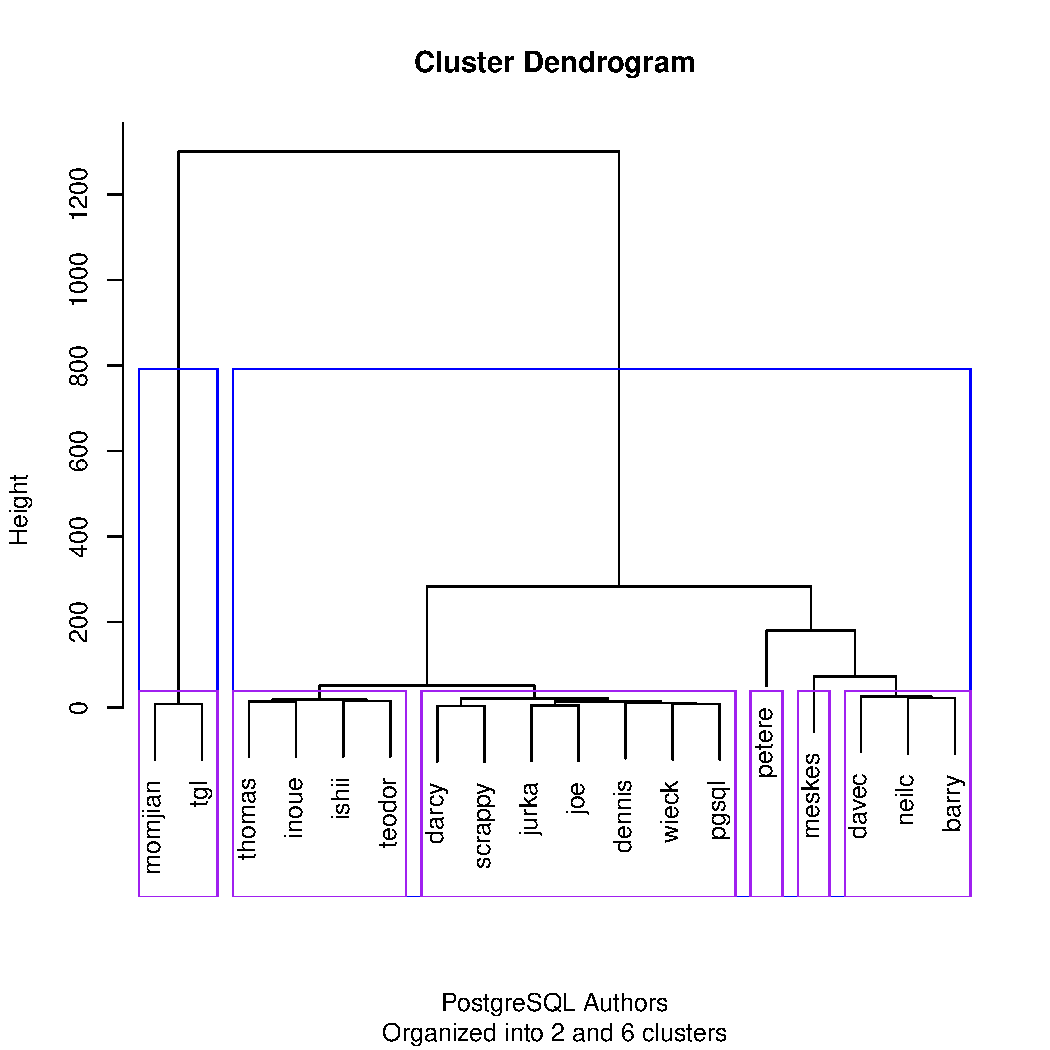
\includegraphics[width=.9\textwidth]{figures/postgresql-author-cluster}
  \caption{PostgreSQL Author Clusters: Authors clustered by cosine
    distance of their NFR contributions. The outer rectangles (blue) reflect the 2-clusters; the inner rectangles (purple) reflect 6-clusters.}
\label{fig:authorcluster}
\end{figure}


Figure \ref{fig:authorcluster} shows that when we use $6$-clusters, 
\texttt{petere}, \texttt{tgl} and \texttt{momjian} form their own individual
clusters (i.e., are distant from one another in the 7-d space). 
%NEIL - not sure the relevance of this ... needs more explaining. --> (they are also the most frequent committers). 
This is
interesting because it means that the important developers are not
committing code that fits the same NFR profile. In terms of the 2-clusters,
 we can see that \texttt{momjian} and \texttt{tgl} are in the
same cluster, but \texttt{petere} is not. The most frequent
committers do not share the same clusters, even at the coarsest level. 
This implies that
developers in this sample do work on different sets of NFRs and have different
software quality focuses.


% NEIL --> Explain the reason why this sentence is included: 
%It should be noted that much of PostgreSQL development originates from
%the project mailing list, and the developers are often pushing integrations. 
If we compare the global NFR distribution (that is, the relative global frequency of each NFR label)
to each author we find that 25\%
 of the authors have a similarity of $0.47$ or less. In other words, for these authors (gathered to the lower left of Figure  \ref{fig:authorsim}),
 their NFR distribution does not match well with the global distribution.
We found that number of commits correlated with an author's similarity to the
global NFR distribution ($0.59$ Pearson), i.e., the variables ``number of topics associated with a developer'' and ``number of commits'' are not discriminative.


\begin{figure}
  \centering
  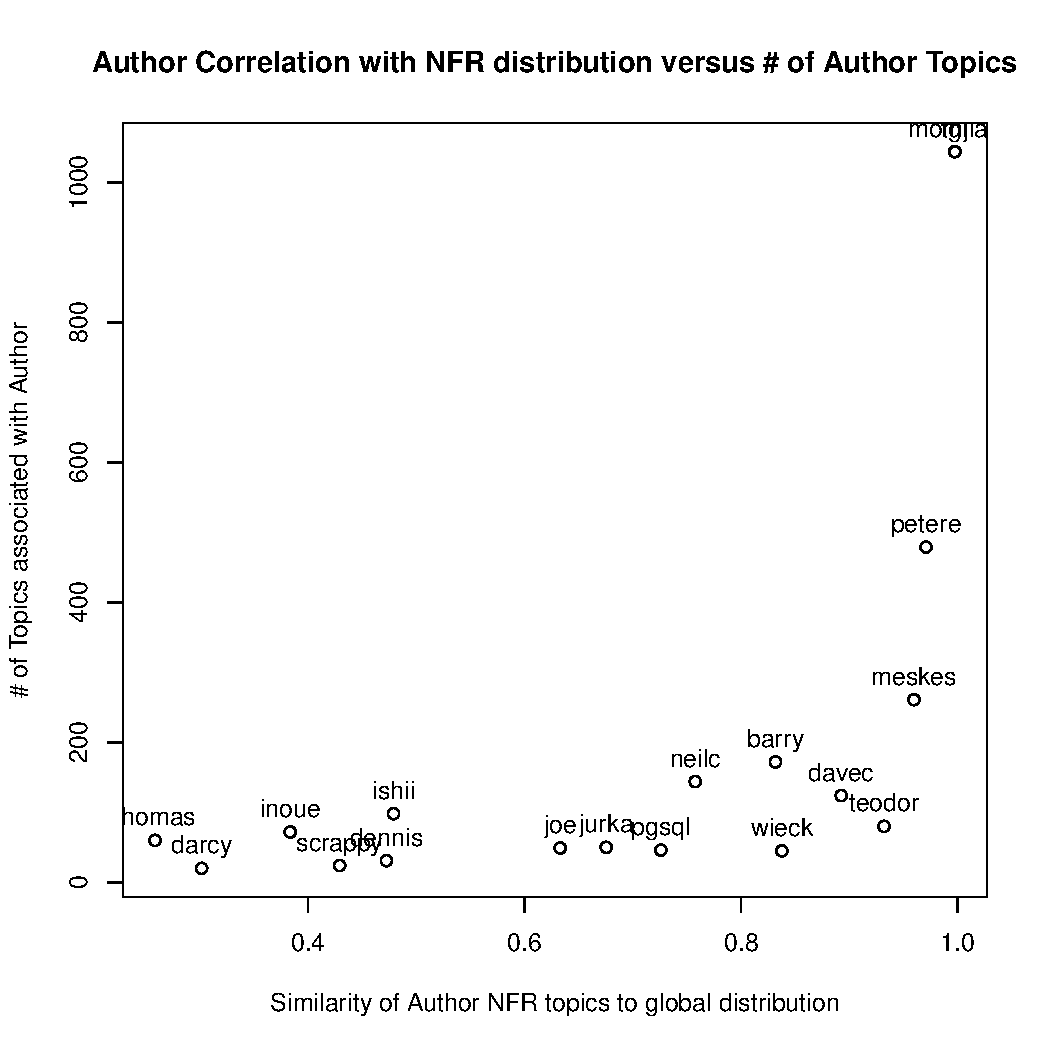
\includegraphics[width=.9\textwidth]{figures/author-distance-from-aggregate}
  \caption{PostgreSQL Author Similarity to the Global Distribution of NFR topics}
\label{fig:authorsim}
\end{figure}


Our working theory is that less frequent committers are more
specialized, e.g., interested in a specific NFR, while the main developers (i.e., frequent committers) either ``wear more hats'' or have more
time to ``wear more hats''. An interesting extension would be to compare this data with 
the PostgreSQL source code files, to see which developer touched which file.

We say that an author (read developer) is ``proportionately interested'' in an NFR if, for all NFRs with which he or she is associated, a given NFR receives the plurality of his or her commits. This is a measure of relative interest and is independent of number of commits (subject to the caveat about frequent committers, above).
If we look at which of the top 15 developers were proportionately interested in a given NFR, we find the associations identified in Table \ref{tbl:devinterest}. Our data also showed that for these top developers, between $1/10$ and $1/3$ of their commits were labelled with a single NFR.

\begin{table}
\begin{tabular}{l|c}
\toprule
\textbf{NFR} & \textbf{Developer} \\
\midrule
\emph{Usability} & \texttt{dennis, neilc} \\
\emph{Portability} & \texttt{scrappy, meskes} \\
\emph{Efficiency} & \texttt{inoue, neilc} \\
\emph{Reliability} & \texttt{jurka, joe} \\
\emph{Functionality} & \texttt{thomas, weick} \\
\emph{Maintainability} & \texttt{scrappy, ishii}\\
\bottomrule
\end{tabular}
	\caption{Developer interest in NFRs}
	\label{tbl:devinterest}
\end{table}


One potential confound for this analysis is that we could be
describing developer style instead of developer focus. Developer style
would be a developer's likelihood to use or not use terms found within
our dictionaries and training corpus in their commit messages. Furthermore, a top developer, in
terms of number of commits, will have more samples, and thus be more likely
take on a more general role. For example, we found in a previous
project~\cite{largechanges} that there was a good correlation between the words used to describe a commit
and the actual author of the commit. 
%were often correlated. Thus based
%on that observation developer style might be a confounding concern.


% Dennis is into usability
% scrappy and meskes portability
% Inoue and neilc for effiency
% jurka joe and barry for Reliabilityb
% thomas weick teodor for Functionality
% ishii, scrappy, darcy for maintainability

%\DONE{Now look at the authors, what are they into?}

% tgl == momjian
% > nauthors
%                     momjian     thomas      davec      neilc      ishii darcy
% None            0.003       0.150       0.048       0.020       0.081       0.15
% Portability     0.211       0.083       0.177       0.173       0.122       0.20
% Efficiency      0.114       0.100       0.080       0.152       0.132       0.00
% Reliability     0.149       0.100       0.137       0.159       0.102       0.15
% Functionality   0.220       0.300       0.266       0.145       0.214       0.20
% Maintainability 0.132       0.150       0.145       0.104       0.224       0.20
% Usability       0.167       0.116       0.145       0.243       0.122       0.10
%                      barry      wieck      inoue      pgsql teodor jurka
% None            0.03488372 0.04444444 0.04166667 0.06521739 0.0250  0.04
% Portability     0.13372093 0.17777778 0.09722222 0.19565217 0.2250  0.18
% Efficiency      0.13372093 0.08888889 0.26388889 0.15217391 0.1250  0.12
% Reliability     0.19767442 0.11111111 0.12500000 0.06521739 0.0875  0.24
% Functionality   0.20930233 0.28888889 0.23611111 0.19565217 0.2375  0.16
% Maintainability 0.13372093 0.06666667 0.13888889 0.17391304 0.1250  0.14
% Usability       0.15697674 0.22222222 0.09722222 0.15217391 0.1750  0.12
%                         tgl    scrappy     petere     dennis     meskes
% None            0.006704981 0.08333333 0.02296451 0.06451613 0.02298851
% Portability     0.207854406 0.25000000 0.20250522 0.22580645 0.23754789
% Efficiency      0.119731801 0.08333333 0.09812109 0.12903226 0.08045977
% Reliability     0.150383142 0.16666667 0.12734864 0.09677419 0.14559387
% Functionality   0.217432950 0.12500000 0.20668058 0.12903226 0.22222222
% Maintainability 0.129310345 0.20833333 0.14196242 0.00000000 0.10727969
% Usability       0.168582375 0.08333333 0.20041754 0.35483871 0.18390805
%                        joe
% None            0.06122449
% Portability     0.22448980
% Efficiency      0.08163265
% Reliability     0.22448980
% Functionality   0.12244898
% Maintainability 0.10204082
% Usability       0.18367347


\section{Discussion}
\label{sec:limit}

\subsection{Annotation Observations}
We found many topics that were not actually non-functional requirements (NFRs) but were often related to them. 
For instance, concurrency was mentioned often in the commit logs and
was related to \emph{correctness} and \emph{reliability}, possibly because concurrent code is prone to bugs such as race conditions. %are 
% often  was troublesome. 
\emph{Configuration management} and \emph{source control} related changes appeared often; % and sometimes there were topics dedicated to configuration
% management. 
these kinds of changes are slightly related to \emph{maintainability}. 
A non-functional change that was not quality-related was licensing and
copyright; many changes concerned updating copyrights or
ensuring copyright or license headers were applied to files. In these
cases we assigned the \emph{None} label to the topic.

We noticed that occasionally the names of modules would conflict with words related to other non-functional requirements. 
For instance, optimizers are very common modules in database systems:
all three projects, MySQL, MaxDB, and PostgreSQL have optimizer modules. 
In MySQL the optimizer is mentioned but often the change addresses  correctness or another quality. 
Despite this difference, the name of the module could fool our learners into believing the change was always about \emph{efficiency}. 
In these cases the advantages of tailoring topic names to specific project terminologies are more clear. 
Project specific word-lists would avoid automated mistakes due to the names of entities and modules of a software project.

\subsection{Inter-rater reliability}
\label{sec:inter-rater}
To determine inter-rater reliability two of the authors---Ernst and Hindle---each annotated the PostgreSQL topics,
and then evaluated each other's annotations.

%>    A_portability   A_functionality     A_reliability A_maintainability
%>      0.153548387      -0.013588517       0.004573794       0.082001031
%>     A_efficiency       A_usability            A_none
%>      0.231496539       0.009287926       0.062133646

% > Spearman says
% >   A_portability   A_functionality     A_reliability A_maintainability
% >      0.253037469      -0.014415214       0.004579664       0.082215613
% >     A_efficiency       A_usability            A_none
% >      0.258037216       0.014436230       0.080667468

\begin{table}
\centering
\begin{tabular}{l|c|c}
\hline
            & Cohen's Kappa & Spearman Correlation \\ \hline
Portability & 0.154 & 0.253  \\
Functionality & -0.014 & -0.014 \\
Reliability & 0.005 & 0.005 \\
Maintainability & 0.082 & 0.082 \\
Efficiency & 0.231 & 0.258 \\
Usability & 0.009 & 0.014 \\
None &      0.062 & 0.081 \\ \hline 
Everything & 0.107 & 0.108 \\ \hline
\end{tabular}
\caption{Inter-rater Reliability on PostgreSQL}
\label{tab:interr}
\end{table}

Table \ref{tab:interr} describes the Cohen Kappa and the Spearman
correlation of our per topic annotations for each NFR. We had to
evaluate inter-rater reliability this way because a single topic could be
tagged with more than one NFR. 

We feel these results are poor. The aggregate view of a Kappa of
$0.1$ indicates there is some weak agreement. We found that
there was a lot of agreement in terms of lack of a tag, but often more
disagreement when a tag should be applied. After some discussion we concluded that usability was a source of
disagreement. Do user manuals improve usability? Is a command-line
option a usability issue? These kinds of questions illustrate some of
the agreement, disagreement and ambiguity about these labels. 
Thus we would recommend that future annotators make a concerted effort
to train and discuss when one applies an annotation.



Empirically how poor were our results? We decided to compare our
results against simulated or random results. In the first simulation
we sampled with replacement from our own NFR label distributions to
produce random ratings that looked like our own. We then applied the
Kappa-statistic on this sampling versus our labelling, and repeated
this 100,000 times, we found that
for 4 out of 7 NFR labels, our labels IRR were greater than the random
IRR measures 96\% of the time. For portability and efficiency, our IRR
was greater 100\% of the time both for Neil's ratings, Abram's ratings
and the union of both Neil and Abram. Figure \ref{fig:irr} depicts the IRR of
these sampled ratings versus our IRR using the Kappa statistic.

We also achieved similar results if the ratings were pulled from a
uniform distributions. What this does indicate is that our labels and
ratings were definitely better than random except for functionality,
reliability and usability. 

\begin{figure}
  \centering
  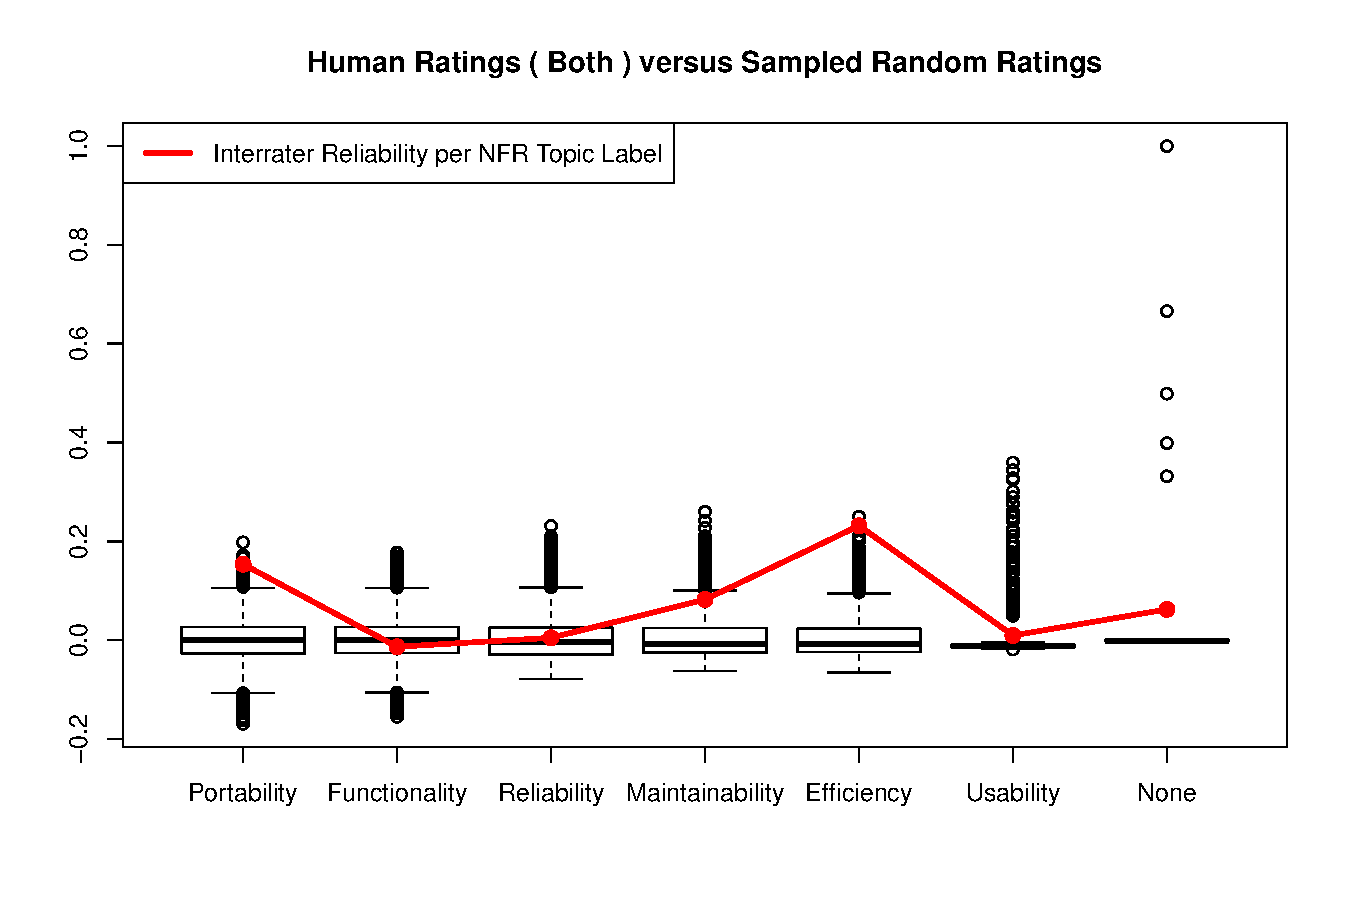
\includegraphics[width=0.9\textwidth]{figures/self-sample-Both}
  \caption{Measured IRR versus IRR of labeling random simulations.}
  \label{fig:irr}
\end{figure}

We feel that this resulting IRR score, although lackluster, indicates
the underlying difficulty of annotating such a data-set.
Consistent training of the annotators (the people) might avoid low IRR scores, or
using more annotators.
Other improvements could be gained by approaching some of the original developers
and using their expertise to annotate the data according to their intent.
Thus improvements
could be gained by producing more robust training samples that use
multiple raters, or experts, who are similarly trained and willing to discuss and
negotiate disagreements.



% [1] "Person  Abram"
% [1]  3.093543e-06  1.269107e-04 -5.132487e-05 -1.449561e-05  7.953201e-05
% [6] -2.791593e-05  6.246161e-05
% [1] "Person ECDF measures Abram"
% [1] 0.99992 0.36418 0.55153 0.97717 1.00000 0.64988 0.96132
% [1] "Person  Neil"
% [1] -1.426950e-04 -8.394072e-06 -1.108948e-04  8.568950e-06 -1.531356e-06
% [6]  3.387974e-05 -9.010485e-05
% [1] "Person ECDF measures Neil"
% [1] 0.99994 0.36777 0.55371 0.97775 1.00000 0.59585 0.92487
% [1] "Person  Both"
% [1] -1.026767e-04  2.685101e-05  2.550572e-06  5.996015e-05 -4.787163e-05
% [6] -1.982510e-04 -8.891684e-05
% [1] "Person ECDF measures Both"
% [1] 0.99995 0.37230 0.57847 0.96622 0.99998 0.90559 0.99859



% I think this is largely due to lack of training. So I will write it up as such - as an interesting point to say that agreeing on the meaning of "software quality" is difficult, etc. Ideally we would now do a sample training session where we go over say one period and determine the appropriate annotations, then recalculate Kappa to see what changes.

% The other tack is to ignore the IRR data completely as we did in the workshop. But I don't think it hurts our results that much ¦ just confirms the difficulty of annotation.

% Neil



\subsection{Summary of Techniques}
While an unsupervised technique such as LDA is appealing in its lack of human intervention, and thus lower effort, 
supervised learners have the advantage of domain knowledge, which typically means improved results. 
% NEIL - we got criticized for making it sound like this is the obvious thing to do... and then why do you need a learner?
%Our manual annotations were fairly quick to do, taking only a few minutes per 30 day period. 
Creating annotated topics (i.e., manual labels) for training is painstaking, but with a suitably representative set of topics, the effort is acceptable. To
annotate \emph{all} topics took us approximately 20 hours per project, but we estimate only 10\% of the topics need annotation to produce useful results.

Very rarely did \textsf{exp2} and \textsf{exp3} (semi-unsupervised word matching) ever perform as well as the supervised machine learners. 
For MaxDB, \textit{reliability} was slightly better detected using the static word list of \textsf{exp2}. 
In general, the machine learners and \textsf{exp3} did better than
\textsf{exp2} for MySQL and MaxDB, yet for PostgreSQL the
\textsf{exp2} word-lists performed better.
For both MySQL and MaxDB \textit{usability} was better served by \textsf{exp2}. 
\textit{Usability} was a very infrequent label, however, which made it difficult to detect for both approaches.

The semi-unsupervised labelling had difficulty distinguishing between common labels and infrequent labels. 
The learners would occasionally mislabel a topic deserving of an infrequent label with a more common label.
The word-lists for \emph{correctness} tended to be too lengthy, non-specific and broad, especially if WordNet words were used, since the NFRs are
typically loosely defined concepts in common parlance.

We found that the multi-label learners of BR, CLR and HOMER only did
as well or worse for Macro-ROC as the single-label Naive Bayes and other naive Bayes-derived learners. 
This suggests that by combining together multiple Naive Bayes learners
we could probably label sets of topics effectively, but it would
require a separate Naive Bayes learner per label.

%{Discuss how these are CHEAP techniques and although somewhat %inaccurate they don't require a tonne of work}

With ROC values ranging from $0.6$ to $0.8$ for MySQL and MaxDB and
$0.47$ to $0.6$ for PostgreSQL, we can see there is promise in supervised methods.
\textsf{exp2} and \textsf{exp3} both indicate that static information can be used to help label topics without any training whatsoever. 
MySQL and MaxDB's machine learners made some decisions based off a few shared words: \textsf{bug, code, compiler, database, HP UX, delete, memory,
missing, problems, removed, add, added, changed, problem, and test}. 
Adding these words to the word-lists of \textsf{exp2} and \textsf{exp3} could improve performance while ensuring they were only domain specific.

If the techniques used in \textsf{exp2} and \textsf{exp3} were combined with the supervised techniques, we could reduce the training effort by boosting
training sets with topics classified with the semi-unsupervised techniques.
Both Naive Bayesian learners and the word-list approaches were computationally efficient.  
%These results are promising, because the accuracy of the techniques is good enough to be useful, while the run-time performance is still cheap enough
%to execute to be feasible as an automated or semi-automated method of
%labelling topics by their software qualities.
Low F-measures and ROC scores are a concern for some of these
techniques, perhaps the word lists need to be re-enforced or made
robust in the face of heavy class imbalance.
These results are promising because they indicate that these
techniques are accurate enough to be useful while still maintaining
acceptable run-time performance.

While this work focuses on labelling natural language commit log
comments, we feel it can be adapted to other natural language software artifacts, 
such as mailing-list discussions and bug reports. Bug reports might not exhibit the same
behaviour as commits in terms of dominant topics.

\subsection{Threats to Validity}
% can always be cut down

Our work faced multiple threats to validity and we attempted to address many of them:

\emph{Construct validity} -- we used only commit messages rather than
mail or bug tracker messages. 
To extend further we would need matching repositories for each project.
%Each case study was BecauseSince we required a seamless record, it was not possible to obtain
%other data sources. 
Possibly they would have influenced our results, but there would be a degree of correlation between the corpora.
 It is possible for a given label to occur across the arbitrary 30-day boundary we set. We suspect but have not proved that this is insignificant. 
%Conversely, construct validity was addressed in our validation as we used the files, topics and revisions to annotate the commit messages. 
%We used mailing-lists to verify the purpose behind some events.
Our taxonomy for software NFRs is subject to dispute, but seems to be
generally accepted.  A future approach should consider a different taxonomy, such as one created by surveying developers on what ``types" of tasks they work on.
Finally, there are exogenous sources, such as
in-person discussions, which we did not access.  %We did not show these results to the stakeholders.

Our word-lists were built up of words that were assumed to be relevant
to those topics, our automated analysis was ignorant of the multi-uses
of words and thus topics could be flagged inappropriately. For
instance, if the word \emph{redundancy} is used would it reference
reliability or cloned code? This issue is why we checked the
performance of the techniques, although we did not explicitly check
for these cases.

Developer style is another confounding issue, if we are searching for
these words we are relying on developers to use these words. This
study might be exploiting the behaviour or style of a few
developers. If one developer did not describe their commits well or
used fewer terms it is likely they would be associated with a NFR
topic regardless of the actual purpose of their commits.

\emph{Internal validity} -- %includes inter-rater reliability and our lack of rival explanation building. 
We improved internal validity by trying to correlate and explain the behaviours observed in the analysis with the historical records of the projects.
We did not attempt to match our results to any particular model.

PostgreSQL's size in terms of commits was equal to MySQL and MaxDB
combined. This imbalance in size, combined with the choice of 20
topics per month produced topics that represented too many issues or
threads within PostgreSQL's development. Choice of number of topics
should probably be tuned to the project.

We primarily relied on ROC (the area under the receiver operating
characteristic curve), as our measurement to compare the effectiveness
of semi-supervised and supervised learners. ROC is less biased than
F-Measure in cross-folds
validation~\cite{flach-icml03,Forman:2010:ACS:1882471.1882479} in the
case of class imbalance. We
feel that the fixed point of $0.5$ for random results allows us to
better describe the predictability achieved by some of these
techniques against random and ZeroR learners. 
We also include
F-Measure results to allow for the reader to validate against
F-Measure if they are more comfortable with it. Thus because of
F-Measure biased handling of class-imbalance and the inherent
class-imbalance that our data suffers from we chose ROC.

%XXX If we have more time try to elaborate more on this
One potential issue with some of our results is that we achieved very
low ROC and F-Measure scores.  Performance was not uniformly low,
often the more common classes exhibited better performance than the
more rare classes.  Often this was amplified by class imbalance. In
future work we plan to investigate techniques such as sub-sampling and
boot-strapping in order to improve performance. Some of the ROC
performance could be due to a lack of coherence in tagging which was
shown by our low inter-rater reliability score.

We assessed inter-rater reliability (IRR), a measure of the correlation between the manual annotations the first two authors created. Perfect IRR (1.0) indicates complete agreement 
on the appropriate annotation for that topic. We verified IRR using
manually annotated PostgreSQL topics, and achieved a weak result of $0.1$.
Some of the reasons for this are a disagreement over the appropriate classification for documentation topics (should this be considered
usability or portability?). A short education session on what a given
NFR from the ISO standard encompasses would reduce this error rate.
Weak IRR results could also be responsible for some the low ROC
performance, if each rater is picking up on different information it
might make it more difficult to train a machine learner to do the
same.
Furthermore weak IRR results threatens the validity of the
experiments, if raters cannot agree then consistently labelling by
ISO-9126 related NFRs could be quite difficult.



\emph{External validity} -- %was addressed by our use of two case studies, but there are still issues. 
Our data originated from OSS database projects and thus might not be applicable to commercially developed software or other domains. 
Furthermore, our analysis techniques rely on a project's use of meaningful commit messages, although we feel this is the most frequently occurring form
of developer comments. 
While we tried to control for application domain variability, OSS
projects investigated were database systems, thus our results might
not generalize well to other domains.


% in Case Study Research: Design Case Studies
\emph{Reliability} -- each annotator, the first two authors, followed the same protocol and used the same annotations. 
However, only two annotators were used; their annotations exhibit some
bias as suggested by the weak inter-rater reliability for
PostgreSQL. Inter-rater reliability could not be checked for MySQL and
MaxDB because annotators did not rate the same documents.

\subsection{Future Work}
There are several avenues of further investigation.  
More external validation would be useful. 
Although we validated our comparisons using a mailing list for each project, interviews with developers would provide more detail. 
We also think multi-label learning techniques, although in their infancy, are crucial in understanding cross-cutting concerns such as NFRs. 
We want to leverage different kinds of artifacts to discover threads of NFR-related discussions that occur between multiple kinds of artifacts.
Finally, we would like to extend this analysis to other domains, to
see what patterns might occur within those domains, such as consumer-facing software products.

\section{Conclusions}
This paper presented a cross-project data mining technique,
\emph{labelled topic extraction}. %The technique leveraged a
%non-functional requirements (NFRs) taxonomy to mine and label latent
%software development topics. 
Previous topic analysis research produced project-specific
topics that needed to be manually labelled.
%, but topics without labels
%are difficult to interpret, and manually labelling them is
%costly. Furthermore, previous work was project-specific and thus incomparable. 
To improve on this, we leveraged software engineering standards,
specifically the ISO9126 quality taxonomy, to produce a method of partially-automated (supervised) and fully-automated (semi-unsupervised) topic labelling.
Since the word-list technique is not project-specific, we used it to compare three distinct projects, where we showed our technique produced interesting
insight into maintenance activity. %topics and artifacts from project histories.
% Our contributions include:
% \begin{itemize}
% \item We provided an unsupervised method of topic labelling (word-lists);
% %\item Our unsupervised method can be applied to projects without training;
% \item We demonstrated a supervised method of labelling topics by a single NFRs (machine learning);
% \item We demonstrated a supervised method of labelling topics by multiple NFRs (multi-label machine learning);
% \item We provided a method of cross-project analysis via topic labelling;
% \item We demonstrated a method of visualizing these topics across time, which we used to analyze maintenance activities.
% \end{itemize}


We validated our topic labelling techniques using multiple experiments. % on unsupervised learners, supervised and multi-label learners. 
We first conducted semi-unsupervised labelling using word-lists. 
Our next approach was supervised, using single-label and multi-label learners. 
Both kinds of learners performed well with average
%area under the 
ROC values between $0.6$ and $0.8$. 
These results were confounded by our low inter-rater reliability score
on the PostgreSQL data-set, suggesting that annotators need careful
and thoughtful training.
With appropriate rigor in annotation, these results, along with the performance of our learners,
demonstrate that labelled topic extraction can be
a promising approach for understanding the occurrence of non-functional requirements in software projects. 
%Although it may seem like common knowledge that maintenance is a concern as a project matures, our technique was able to show this independently.
%We showed that NFRs are often trending topics in commit comments
%, and that NFRs are quite common as developer topics.
%; and that there are efficient methods of automating topic labelling.

%%%HMMM

Our data and scripts are available at \url{http://softwareprocess.es/nomen/}

% We demonstrated multiple supervised and unsupervised methods of topic labelling, including multi-label learners.
% We provided a case study and visualization of NFR related topics in MaxDB 7.500 and MySQL 3.23. 
% During the case study we manually labelled hundreds of topics by hand and then used these annotations to validate the positive performance of topic
%labelling techniques.
% The implication of our paper is that topics with labels are more useful for analyzing software development activities than are unlabelled topics. To
%furnish stakeholders with labelled topics, our technique provides many methods of automatic topic labelling.

% 
% \begin{acknowledgements}
% 	Thanks to the helpful comments from the external reviewers.
% \end{acknowledgements}

% BibTeX users please use one of
%\bibliographystyle{spbasic}	  % basic style, author-year citations
\bibliographystyle{spmpsci}	 % mathematics and physical sciences
%\bibliographystyle{spphys}	  % APS-like style for physics
\bibliography{ese}   % name your BibTeX data base

\end{document}
% end of file template.tex

